\section{Configuration des \textit{benchmarks}}
\subsection{Simulations effectuées}
Ce chapitre analyse les performances obtenues par l'implémentation \acs{GPU} et hybride (Palabos) et les paramètres qui les affectent. Les \textit{benchmarks} sont réalisés avec deux programmes différents qui utilisent la bibliothèque \texttt{lbmcuda} (l'implémentation Cuda): \texttt{lbm\_simple\_lbmcuda} et \texttt{cavity\_benchmark}.

Le premier simule le même type de problème que \texttt{lbm\_simple} (voir section \ref{title-implementation_python_C}) avec ou sans transfert des populations à chaque itération afin de mesurer les performances sur \acs{GPU}. Le second, décrit en section \ref{title-cavity_benchmark}, simule un écoulement dans une cavité pour évaluer les performances d'une configuration hybride \acs{CPU}/\acs{GPU} avec Palabos.  

\subsection{Matériel utilisé}
Les mesures sont effectuées sur les \acs{GPU} et \acs{CPU} listés dans la table \ref{table:gpu_specs} pour évaluer l'impact sur les performances de plusieurs types de matériel. Le \acs{GPU} utilisé est indiqué sur les mesures ou dans la section qui les présentent. Si rien n'est indiqué, c'est le \acs{GPU} Pascal qui est utilisé.

\begin{table}[h]
\label{table:gpu_specs}
\renewcommand{\arraystretch}{1.3}
\begin{tabular}{|>{\columncolor{gray!25}}l|c|c|c|}
	\hline 
	\rowcolor{gray!25}
	& Pascal & Titan & Tesla \\ 
	\hline 
	Carte NVIDIA & TESLA P100 & TITAN X & TESLA M2090 \\ 
	\hline 
	Architecture & Pascal & Pascal & Tesla \\ 
	\hline 
	Fréquence maximum (MHz) & 1480 & 1531 & 1300 \\ 
	\hline 
	Type de mémoire & HBM2 & GDDR5 & GDDR5 \\ 
	\hline 
	Bande passante mémoire (Go/s) & 549 & 480.3 & 177.6 \\ 
	\hline 
	Perf. simple précision (Tflops) & 10609 & 10157 & 1331.2 \\ 
	\hline 
	Perf. double précision (Tflops) & 5304 & 317 & 665.6 \\ 
	\hline 
    Mémoire globale (MBytes)& 12194 & 12190 & 5301 \\ 
	\hline 
     Nombre de \acs{SM} & 56 & 28 & 16 \\ 
	\hline 
     \acs{SP} par \ac{SM} & 64 & 128 & 32 \\ 
	\hline  
%	\multicolumn{4}{l}{\textbf{Machine hôte}} \\
    \hline
	\acs{CPU}  Intel\textregistered~Xeon\textregistered  & E5-2630 v4 & E5-2643 v3 & X5650 \\ 
	\hline 
	Fréquence du \acs{CPU} (MHz) & 2200 & 3400 & 2670 \\ 
	\hline 
\end{tabular} 
\caption{Spécifications du matériel \cite{ZZZweb_list_2018} utilisé pour les \textit{benchmarks} }
\end{table}

\subsection{Limitations mémoire pour les simulations \acs{LBM}}
Les dimensions du domaine simulé sont limitées par la mémoire du \acs{CPU} et du \acs{GPU}, les simulations étant très gourmandes en mémoire. En effet, les populations du domaine sont allouées au moins une fois sur le \acs{CPU} pour les transferts et surtout trois fois en mémoire globales sur le \acs{GPU}: une fois avec $f^\mathrm{palabos}$ pour les transferts et réorganisations mémoire entre \acs{CPU} et \acs{GPU} (section \ref{title-strategie_reorganisation}), puis deux pour la simulation avec $f^\mathrm{in}$ et $f^\mathrm{out}$. Chaque population occupe $f_\mathrm{size}$ octets en mémoire:
\begin{equation}
f_\mathrm{size} = 8 \times Nx \times Ny \times Nz \times 19 
\end{equation}
avec $8$ étant le nombre d'octets d'un nombre flottant en double précision, $Nx$, $Ny$ et $Nz$ les dimensions du domaine et 19 le nombre de directions d'une population D3Q19. Ainsi, les trois populations d'une simulation d'un domaine cubique de dimensions $256^3$ occupent $8 \times 256^3 \times 19 \times 3$ octets soit environ $7.65$ Go en mémoire globale.

Si l'on y ajoute les vélocités, dont la transmission est également prévue, on peut leur additionner $\nu_\mathrm{size}$ octets:
\begin{equation}
\nu_\mathrm{size} = 8 \times Nx \times Ny \times Nz \times 3
\end{equation}
avec $3$ le nombre de dimensions en D3Q19; soit encore environ 402.6 Mo de plus, pour arriver à un total d'environ $8.05$ Go pour un domaine de dimensions $256^3$.

\section{\textit{Benchmarks} des \acs{GPU}} \label{title-benchmark_gpu}

\subsection{Bande passante et débits de transfert}
Cette section présente les mesures des débits d'accès à la mémoire globale et des transferts entre \acs{CPU} et \acs{GPU}. Elles ont été collectéee avec la méthode proposée par \cite{ZZZweb_how_2012}.

Les premières, illustrées sur la figure \ref{fig:bandwidth}, montrent les bandes passantes effectives mesurées (l'accès à la mémoire globale sur le \acs{GPU}). La progression en fonction de la quantité des données copiées est due au fait que le nombre de \textit{threads} capables de copier les données en parallèle évolue jusqu'à ce que la limite de \textit{threads} soit atteinte. Les mesures confirment les bandes passantes théoriques de la table \ref{table:gpu_specs}, les valeurs effectives étant usuellement entre $75\%$ et $85\%$ des bandes passantes théoriques.

\begin{figure}[h]
	\centering
	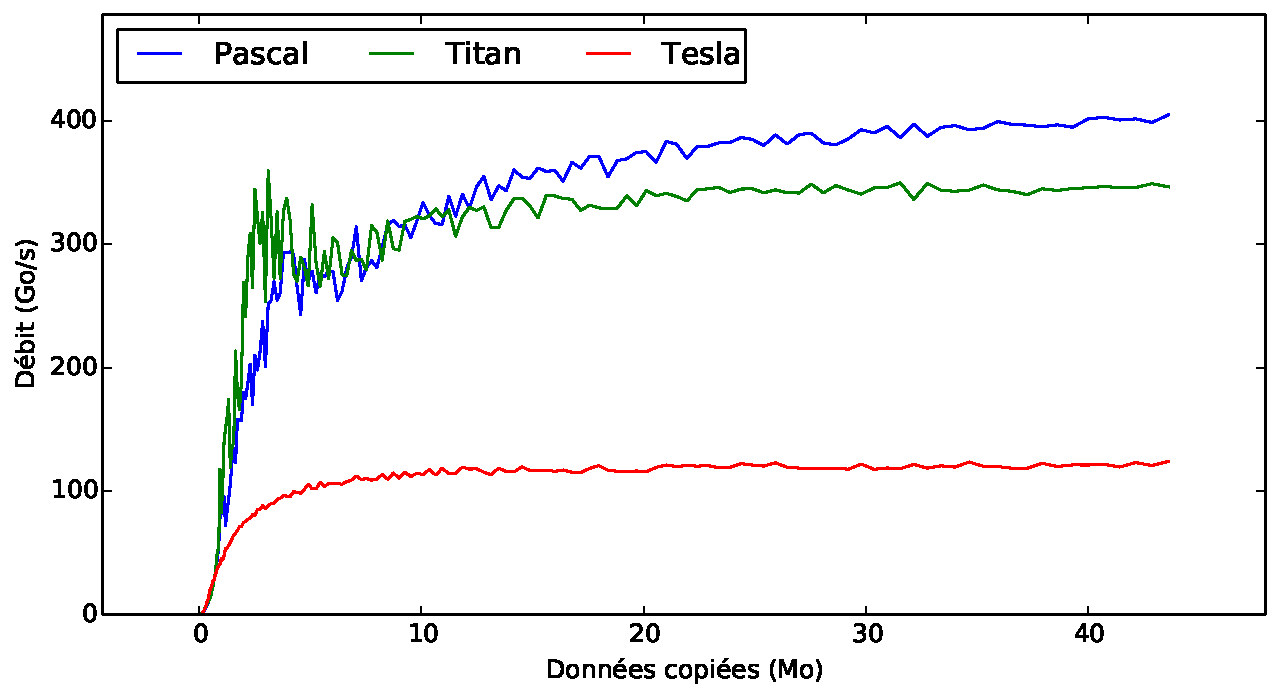
\includegraphics[fbox, scale=0.61]{images/perfs/throughput/bandwidth.pdf}
	\caption{Bande passante effective}
	\label{fig:bandwidth}
\end{figure}

Les secondes mesures, illustrées par la figure~\ref{fig:cudamemcpy_throughput}, montrent les débits de transfert entre le \acs{GPU} et le \acs{CPU} avec \texttt{cudaMemcpy} dans un sens et dans l'autre. On observe la même tendance avec Pascal et Titan et un débit nettement inférieur et plus instable avec Tesla.

\begin{figure}[h]
	\centering
	\subfigure[\acs{GPU} Pascal]{%
		\centering
		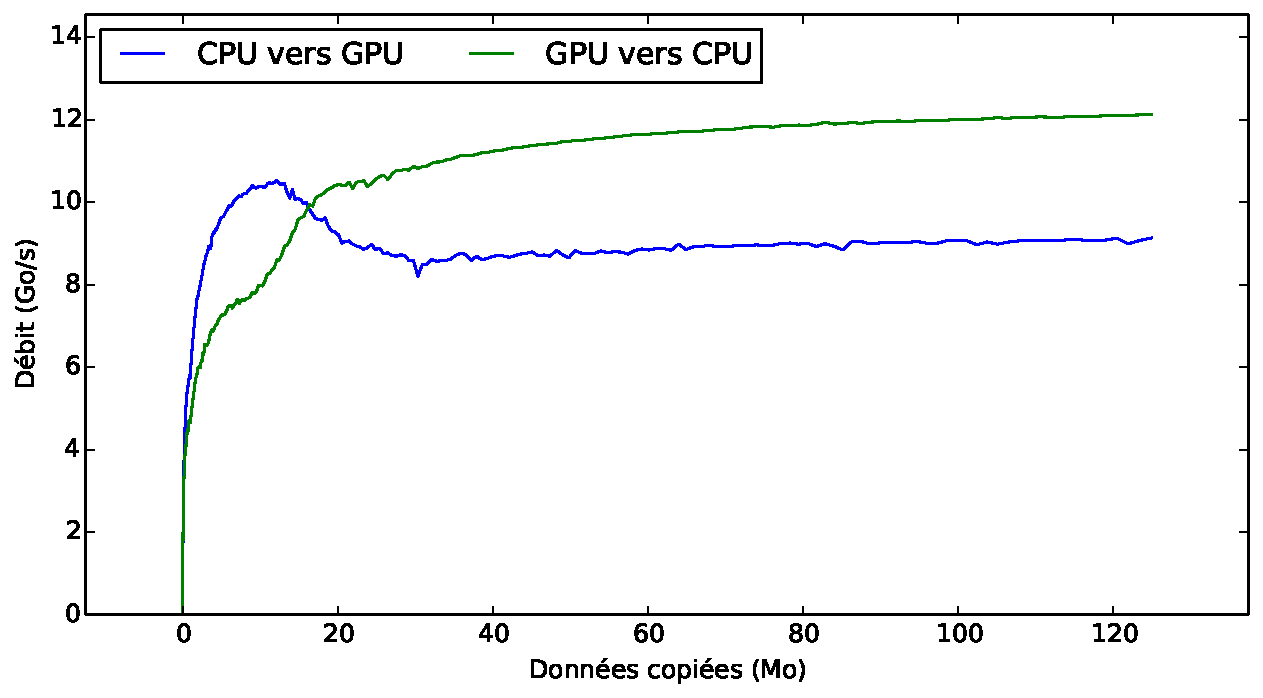
\includegraphics[fbox, scale=0.6]{images/perfs/throughput/data_trsf_pascal.pdf}
	}
	\subfigure[\acs{GPU} Titan]{%
		\centering
		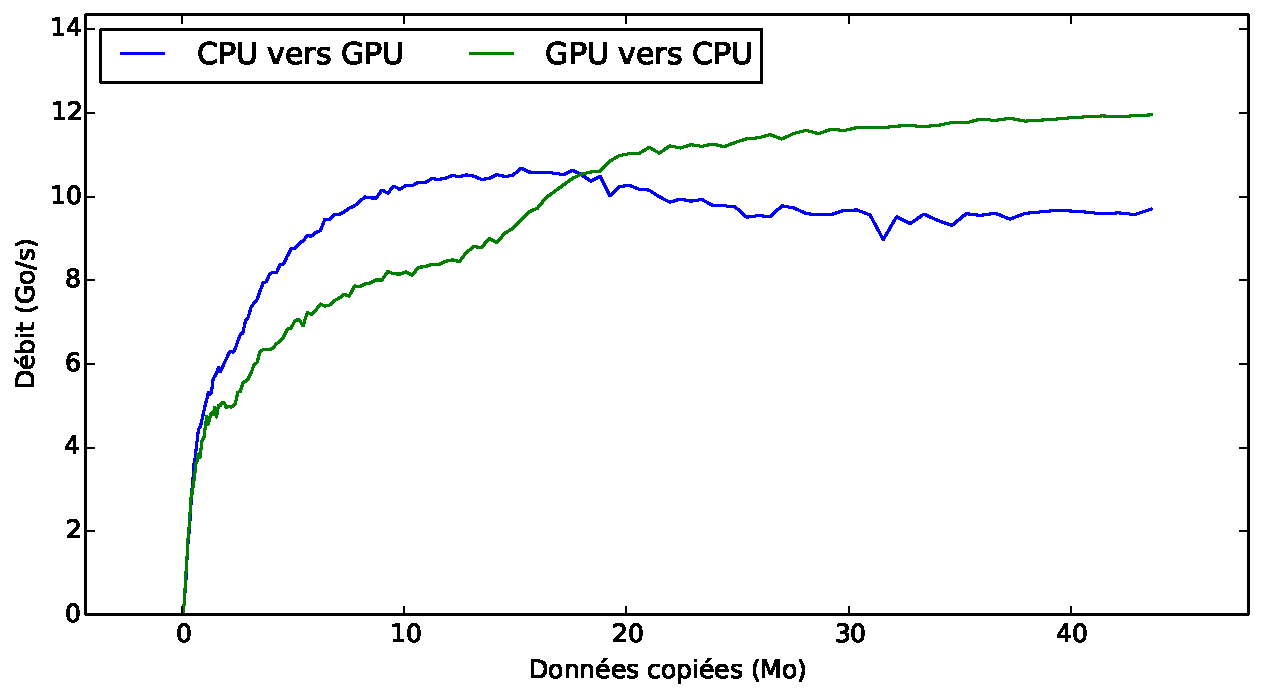
\includegraphics[fbox, scale=0.6]{images/perfs/throughput/data_trsf_titan.pdf}
	}
	\subfigure[\acs{GPU} Tesla]{%
		\centering
		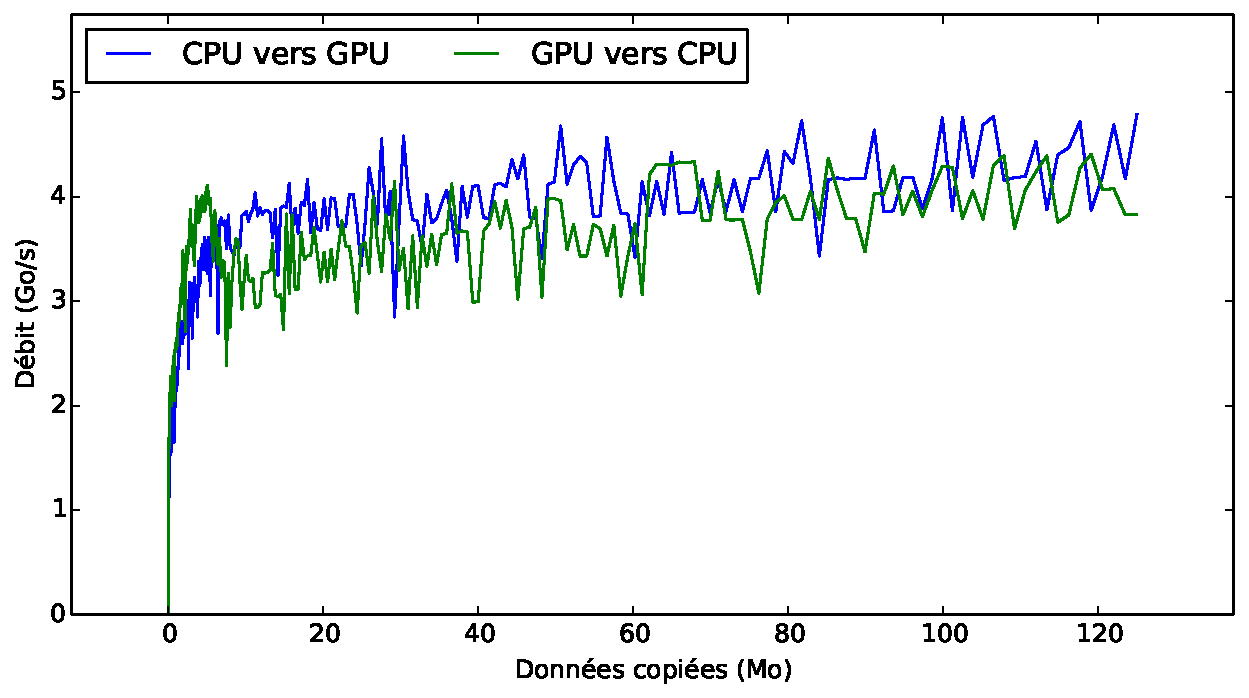
\includegraphics[fbox, scale=0.6]{images/perfs/throughput/data_trsf_tesla.pdf}
    }
	\caption{Débit des transferts entre \acs{GPU} et \acs{CPU} (\texttt{cudaMemcpy})}
	\label{fig:cudamemcpy_throughput}
\end{figure}

\subsection{\textit{Overhead} de lancement d'un \textit{kernel} et latence des transferts} \label{title-latences}

Comme l'illustre la table \ref{table:latence}, l'exécution d'un \textit{kernel} sur le \acs{GPU} ou d'un transfert de données avec \texttt{cudaMemcpy} n'est pas immédiate. Pour mesurer la latence du démarrage d'un \textit{kernel}, on mesure simplement le temps d'exécution d'un \textit{kernel} vide (sans aucune instruction). Pour la latence d'un transfert opéré avec \texttt{cudaMemcpy}, on ne peut pas simplement faire une copie de 0 octet.

Si on considère le temps de transfert $T_{trans} = T_{lat} + \nicefrac{N}{bw}$, avec $T_{lat}$ la latence, $N$ la quantité de données à transférer et $bw$ la bande passante, comme le propose \citet{albuquerque_performance_2012}, il est possible de déduire $T_{lat}$. On mesure le temps d'exécution $T_{trans}$ pour un transfert avec $N$ données puis un second temps de transfert $T'_{trans}$ mesuré pour $m\cdot N$ données et on calcule ensuite $T_{lat}$ ainsi:

\begin{align}
T_{lat} = \frac{ m \cdot T_{trans} - T'_{trans}}{m-1} = \frac{\bigg(m \Big( T_{lat} + \frac{N}{bw}\Big) - T_{lat} + \frac{m\cdot N}{bw} \bigg)}{m-1} = \frac{(m-1) T_{lat} }{m-1}\
\end{align}


\begin{table}[H]
	\label{table:latence}
	\renewcommand{\arraystretch}{1.3}
	\centering
\begin{tabular}{|>{\columncolor{gray!25}}l|c|c|c|}
	\hline 
	\rowcolor{gray!25}
	\multicolumn{1}{|c|}{} 
	& \multicolumn{1}{c|}{Pascal} 
	& \multicolumn{1}{c|}{Titan} 
	& \multicolumn{1}{c|}{Tesla}\\
	\hline 
	Lancement d'un Kernel $[\mu s]$& $4.4$  & $3.552$  & $5.07$ \\ 
	\hline 
	Lancement d'un transfert  $[\mu s]$ & $ 30-50$ & $ 46-75$ & $ 580-640$  \\ 
	\hline 
\end{tabular} 
	\caption{Latences du \textit{kernel} et des transferts avec \texttt{cudaMemcpy}}
\end{table}





\section{\textit{Benchmarks} de l'implémentation \acs{GPU}}

\subsection{Ordre des indices}

Les populations sont conservées dans 19 tableaux en mémoire globale (un par direction). Comme sur \acs{CPU}, l'ordre des indices x, y et z a un impact important sur les performances pour des questions de cache. En effet, les populations sont accédées à une adresse x différente par chaque \textit{thread}, c'est donc l'indice qui change le plus rapidement. Pour profiter au mieux des mécanismes de cache, il faut que les zones mémoire accédées consécutivement soient très proches les unes des autres.

La formule suivante calcule un indice à une dimension, avec $i$, $j$ et $k$ étant chacun l'un des indices $x$, $y$ ou $z$ et $I$, $J$ et $K$ la taille de la dimension de l'indice.
\begin{equation}
indice = (i+I) \bmod I + \Big((j+J) \bmod J + ( k+K) \bmod K \times J\Big) \times I
\end{equation}

Par conséquent, $J \times I$ individus séparent $k$ et $k+1$ , $J$ individus séparent $j$ et $j+1$ mais $i$ et $i+1$ eux sont voisins en mémoire. Il faut par conséquent attribuer $i$ à l'indice qui change le plus rapidement, soit $x$. Cette conclusion est confirmée par les mesures illustrées par la figure \ref{fig:index_order}. Plus les individus indexés par $x$ sont distants, plus les performances se dégradent.
 
\begin{figure}[H]
	\centering
	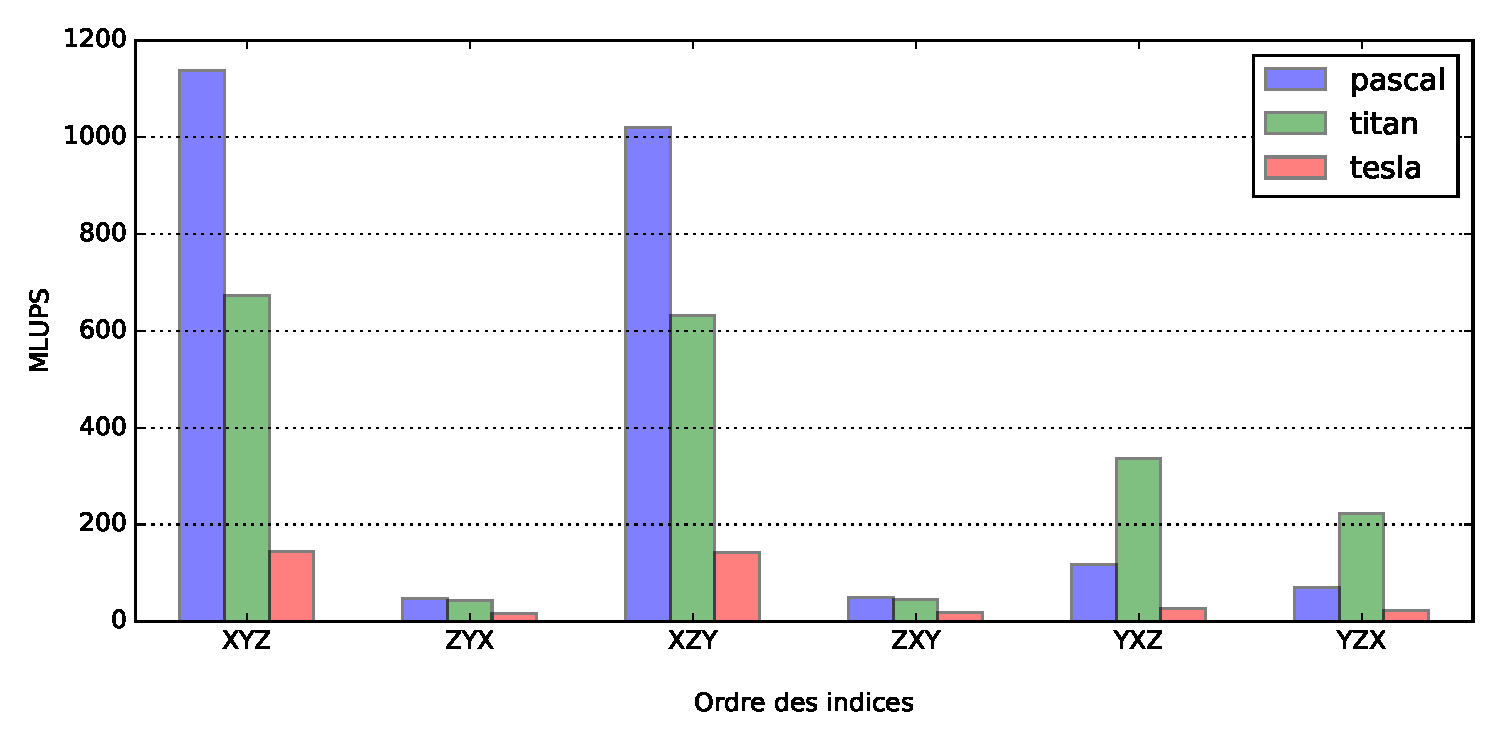
\includegraphics[fbox, scale=0.61]{images/perfs/lbm_simple_lbmcuda/index_order.pdf}
	\caption{Performances en fonction de l'ordre des indices}
	\label{fig:index_order}
\end{figure}

Les meilleures performances sont atteintes avec $i=x$, $j=y$ et $k=z$. Cependant, les \textit{benchmarks} des sections suivantes utilisent $i=x$, $j=z$ et $k=y$. Ce choix est dû à une mesure, effectuée précédemment sur une carte Titan, qui suggérait à tort un très léger gain de performance avec cette configuration.

\subsection{Taille du domaine}
Les figures~\ref{fig:domain_size_bs32} et \ref{fig:domain_size_bs64} montrent que les dimensions du domaine de recherche ont un impact plus ou moins important en fonction du \acs{GPU} utilisé. Sur la figure~\ref{fig:domain_size_bs64}, à l'exception de $192^3$, des pics de performances sont généralement atteints avec les domaines de dimensions multiples de 32 et surtout 64, puis immédiatement suivis d'une chute importante des performances. On observe ainsi une corrélation avec la taille des \textit{warp} (32) et des blocs (64) qui explique probablement en partie cette tendance. Cette supposition est confirmée par la figure~\ref{fig:domain_size_bs32}, qui utilise des blocs de 32 \textit{threads}. On observe dans ce cas des pics identiques sur les domaines aux dimensions multiples de 32.

L'impact de la taille du domaine par rapport à celle des \textit{warp} et surtout des blocs est certainement dû à une moindre utilisation des capacités du \acs{GPU} lors du calcul des derniers blocs. En effet, si les dimensions du domaine de recherche ne sont pas multiples des critères mentionnés, certains \textit{threads} n'ont plus de données à calculer. Leur puissance de calcul est par conséquent perdue jusqu'à l'itération suivante.

\begin{figure}[H]
	\centering
	\subfigure[Blocs de 64 threads]{%
		\centering
		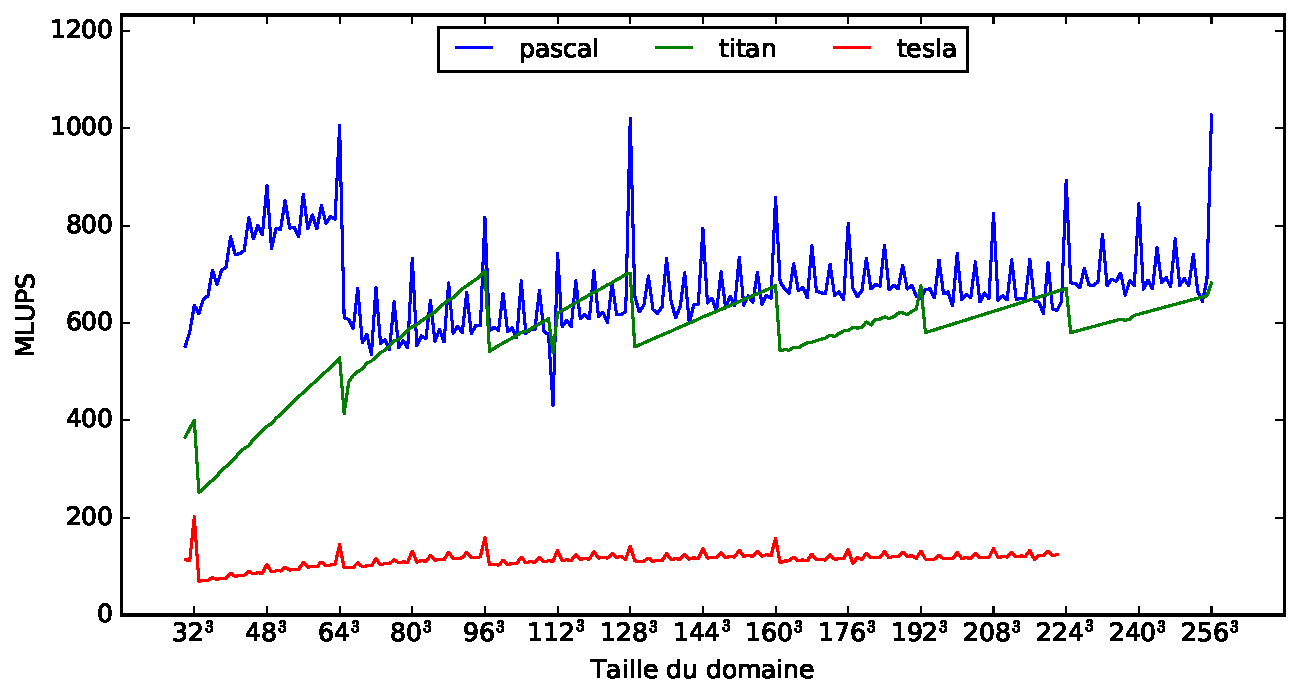
\includegraphics[fbox, scale=0.6]{images/perfs/lbm_simple_lbmcuda/domain_size_bs64.pdf}
		\label{fig:domain_size_bs64}
	}
	\subfigure[Blocs de 32 threads]{%
		\centering
		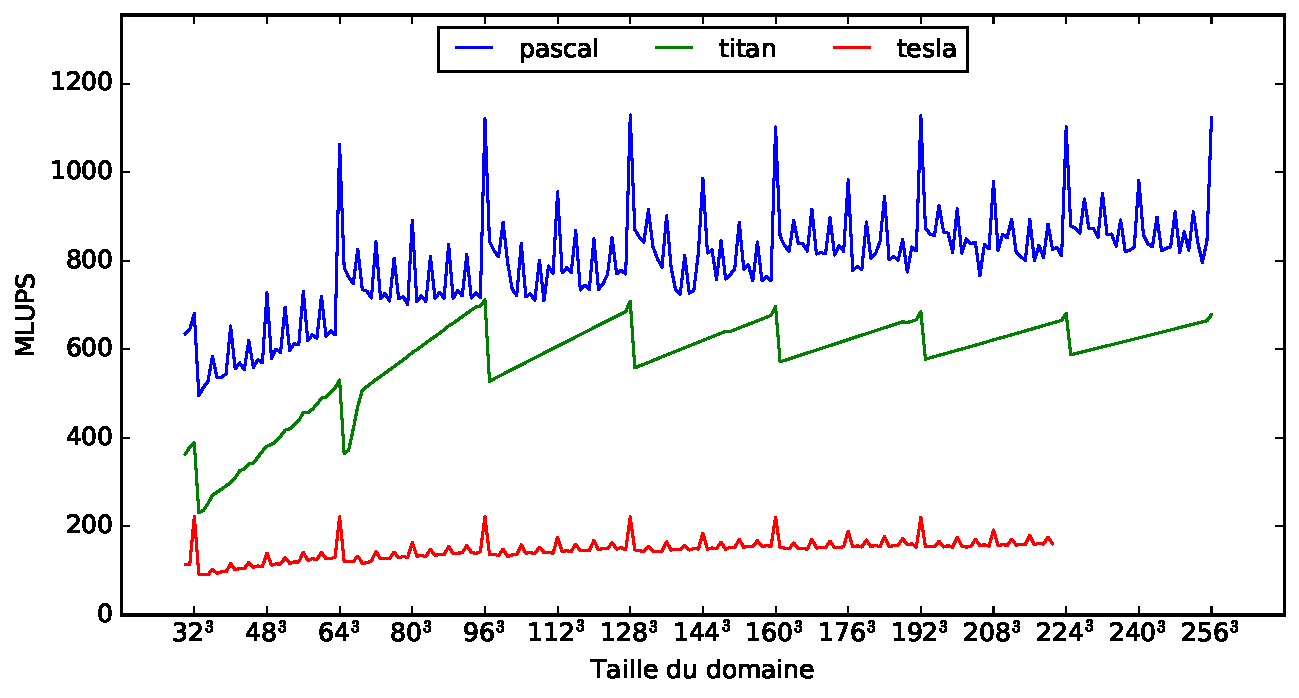
\includegraphics[fbox, scale=0.6]{images/perfs/lbm_simple_lbmcuda/domain_size_bs32.pdf}
		\label{fig:domain_size_bs32}
	}
	\caption{Performances en fonction de la taille du domaine}
	\label{fig:domain_size_bs}
\end{figure}

Les mesures illustrées par figure \ref{fig:lups_by_iter} révèlent une tendance relative à la taille du domaine. Plus le domaine est grand, plus les performances sont stables. En effet, on observe des différences de performances allant jusqu'à plus de 90 \XLUPS{M} pour un domaine de $128^3$ \textit{lattices}, plus de 60 \XLUPS{M} pour un domaine de $64^3$ \textit{lattices} mais presque aucune après 50 itérations sur un domaine de $256^3$ \textit{lattices}.

\subsection{Taille des blocs}
La section précédente met déjà en lumière l'importance de la taille des blocs. Les mesures illustrées par la figure~\ref{fig:lups_by_bs} cherchent à déterminer une taille optimale en fonction de dimension de domaine optimale (multiple de 32). Pour s'approcher du cas hybride, les performances sont désormais relevées sur des mesures qui simulent les transferts \acs{CPU}/\acs{GPU} de Palabos.

On observe des pics de performances pour les tailles de bloc multiples de 32 sur tous les types de \acs{GPU} et, à moindre mesure, les multiples de 16. Toutefois, les meilleures performances sont invariablement observées pour les blocs de 32 \textit{threads}, suivis d'assez près par 64. Cette tendance s'explique probablement par la taille des \textit{warp} qui est identique (32) et que le \acs{GPU} ne peut pas exploiter ses capacités au mieux et atteindre la meilleure \textit{occupancy}  \cite{ZZZweb_achieved_2018} si ces valeurs ne coïncident pas. 

\begin{figure}[h]
	\centering
	\subfigure[\acs{GPU} Pascal]{%
		\centering
		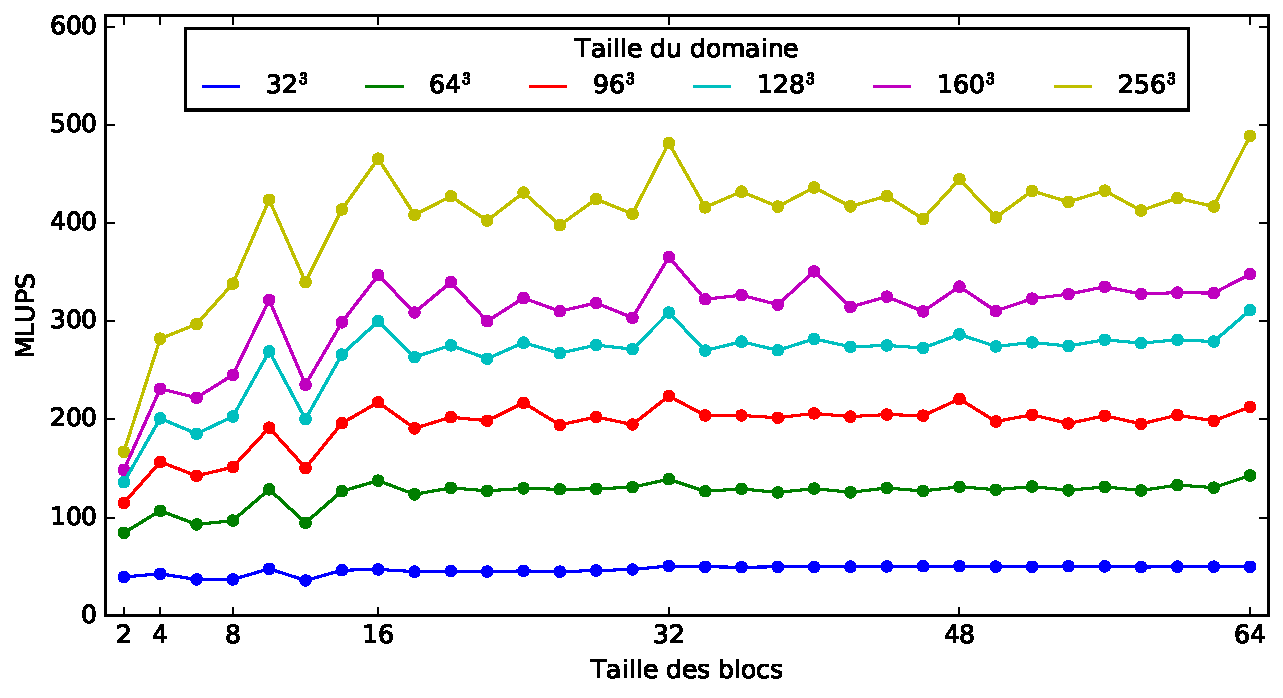
\includegraphics[fbox, scale=0.55]{images/perfs/lbm_simple_lbmcuda/lups_by_bs/pascal_by_bs.pdf}
		\label{fig:lups_by_bs_pascal}
	}
	\subfigure[\acs{GPU} Titan]{%
		\centering
		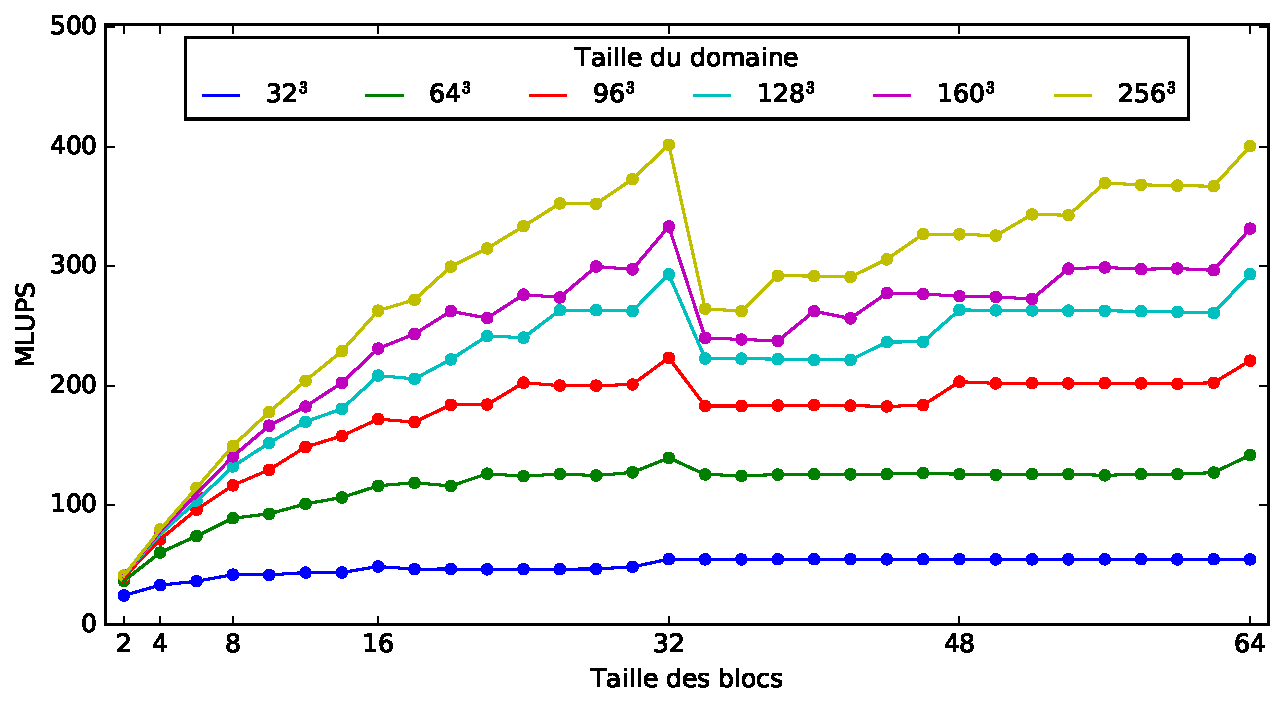
\includegraphics[fbox, scale=0.55]{images/perfs/lbm_simple_lbmcuda/lups_by_bs/titan_by_bs.pdf}
		\label{fig:lups_by_bs_titan}
	}
	\subfigure[\acs{GPU} Tesla]{%
		\centering
		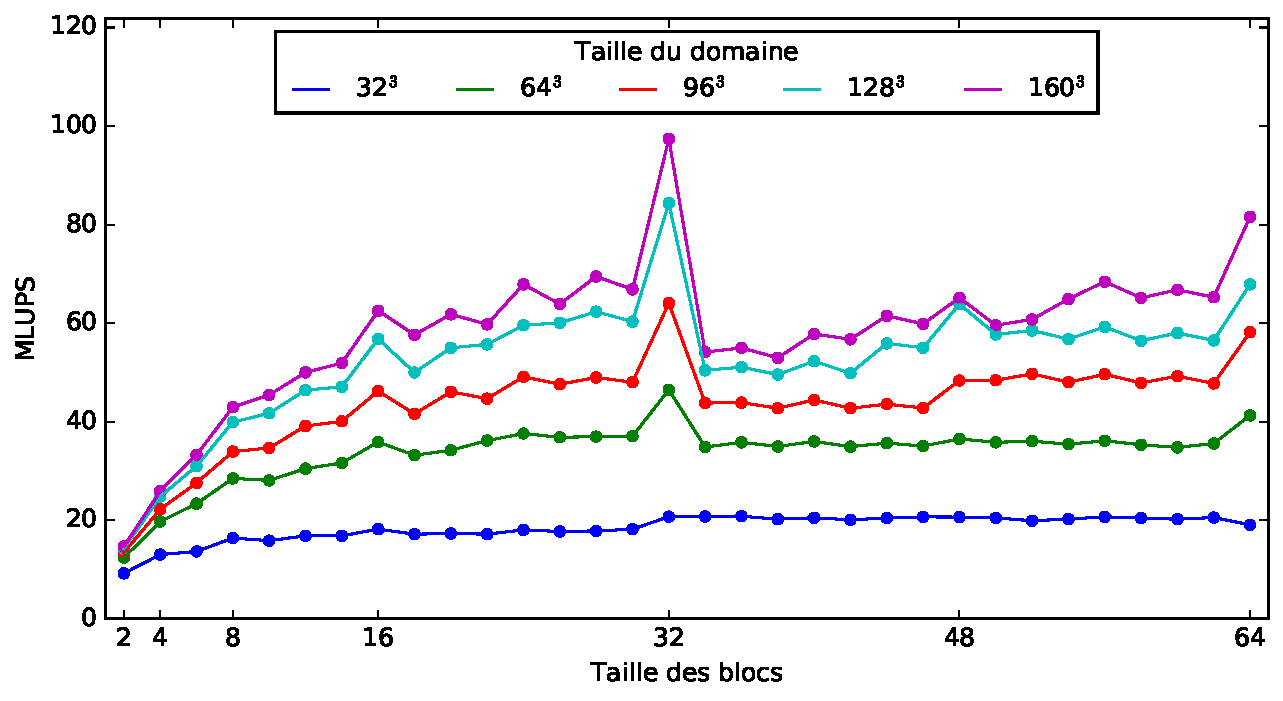
\includegraphics[fbox, scale=0.55]{images/perfs/lbm_simple_lbmcuda/lups_by_bs/tesla_by_bs.pdf}
		\label{fig:lups_by_bs_tesla}
	}
	\caption{Performances en fonction de la taille des blocs}
	\label{fig:lups_by_bs}
\end{figure}

\subsection{Nombre d'itérations}\label{title-iterations}

La figure \ref{fig:lups_by_iter} illustre l'évolution des performances en fonction du nombre d'itérations (ou générations) exécutées, sur trois tailles de domaine différentes ($256^3$, $128^3$ et $64^3$). On observe une brève progression sur les toutes premières itérations, sur la plupart des mesures, certainement due aux initialisations et phénomènes de cache. Par la suite, les performances restent sans surprise relativement stables (sans tendance à la hausse ni à la baisse). Elles sont toutefois bien plus stables lorsque le domaine est grand. 

\begin{figure}[H]
	\centering
	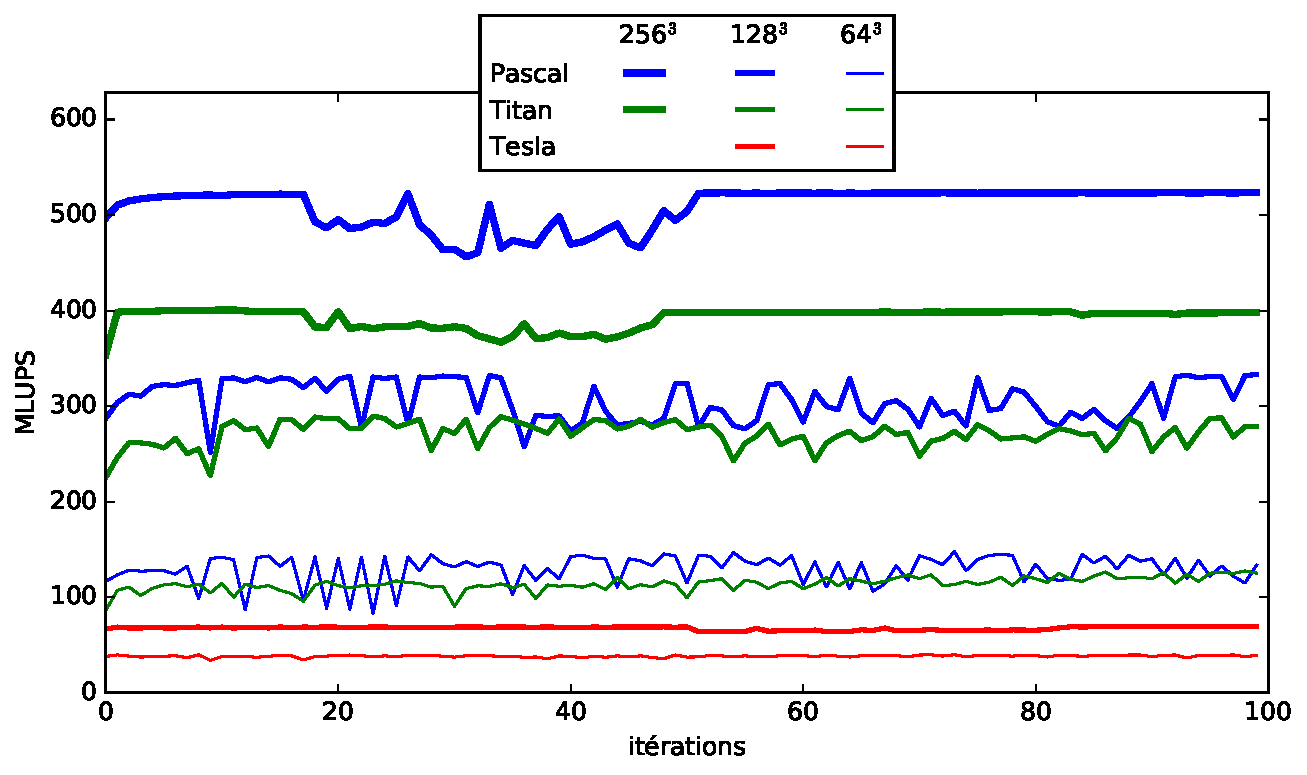
\includegraphics[fbox, scale=0.61]{images/perfs/lbm_simple_lbmcuda/lups_by_iter.pdf}
	\caption{Performances en fonction du nombre d'itérations}
	\label{fig:lups_by_iter}
\end{figure}

\subsection{Profilage} \label{title-profilage_gpu}
Les \textit{benchmarks} des sections précédentes se basent déjà sur des mesures qui simulent les transferts des populations entre le \acs{GPU} et le \acs{CPU} à chaque itération. Cette section s'intéresse à l'impact des trois principales étapes d'une exécution sur \textit{GPU} soit les transferts \textit{Send} (à destination du \acs{GPU}) et \textit{Receive} (à destination du \acs{CPU}) ainsi que les calculs de l'itération \textit{Collide \& Stream}.
	
Les temps d'exécution sont extraits en deux étapes. Une première série de mesures, pour chaque dimension du domaine, est exécutée afin d'extraire un temps d'exécution de référence $T_{0}$. Une seconde série est ensuite exécutée et extrait un temps $T_{1}$ pour l'étape dont on souhaite caractériser. Cette fois cependant, l'étape est artificiellement exécutée $n$ fois (avec $n=10$ dans le cas présent). 

Les temps d'exécution $T_{0}$ et $T_{1}$ sont composé de $T_{send}$, $T_{receive}$ et $T_{collide \& stream}$ (les temps $T_{step}$ possibles) ainsi que d'un temps restant $T_{\epsilon}$ non qualifié:

\begin{equation}
T_{0} = T_{send} + T_{receive} + T_{col \& stream} + T_{\epsilon}
\end{equation}
\begin{equation}
T_{1} = T_{0} + T_{step} \times (n-1)
\end{equation}

\noindent On peut ainsi calculer le temps d'exécution de l'étape $T_{step}$  avec la formule suivante:

\begin{equation}
T_{step} = \frac{T_{0} - T_{1}}{n-1}
\end{equation}

Cette méthode permet d'extraire les temps illustrés par les figures~\ref{fig:gpu_rep_times} et \ref{fig:gpu_curve_times} où l'on observe que le \textit{Collide \& Stream} prend environ autant de temps que les transferts \textit{Send} et \textit{Receive} cumulés. La figure~\ref{fig:gpu_curve_times} illustre l'évolution des temps d'exécution en fonction de la taille du domaine sur une échelle linéaire.

\begin{figure}[h]
	\centering
	\subfigure[\acs{GPU} Pascal]{%
		\centering
		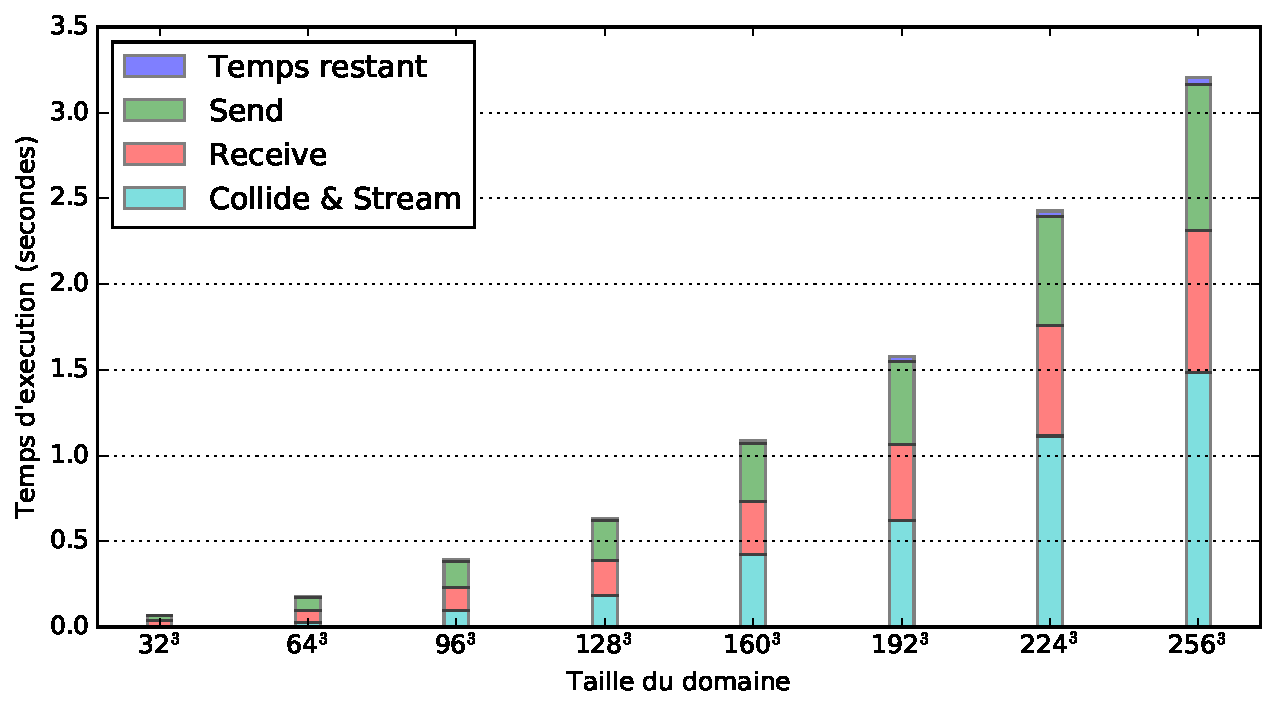
\includegraphics[fbox, scale=0.57]{images/perfs/lbm_simple_lbmcuda/time/repartition/pascal-opt-64.pdf}
		\label{fig:gpu_rep_times_pascal}
	}
	\subfigure[\acs{GPU} Titan]{%
		\centering
		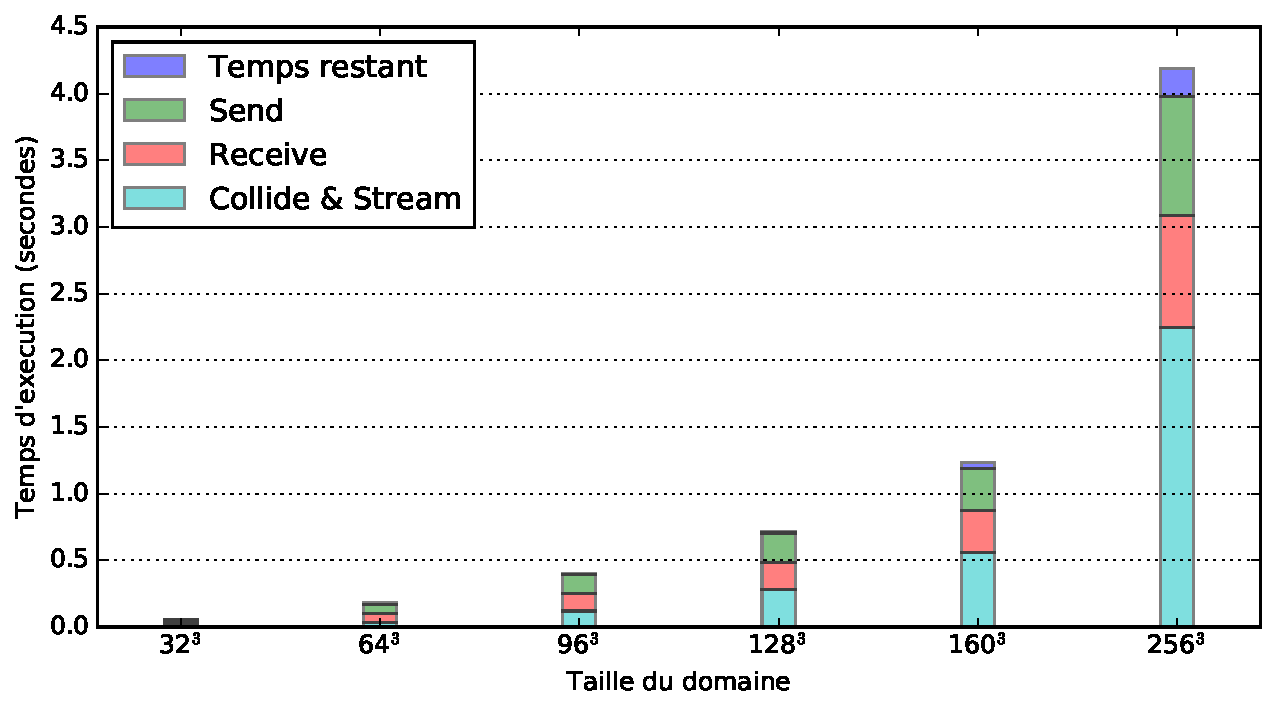
\includegraphics[fbox, scale=0.57]{images/perfs/lbm_simple_lbmcuda/time/repartition/titan-opt-64.pdf}
		\label{fig:gpu_rep_times_titan}
	}
	\subfigure[\acs{GPU} Tesla]{%
		\centering
		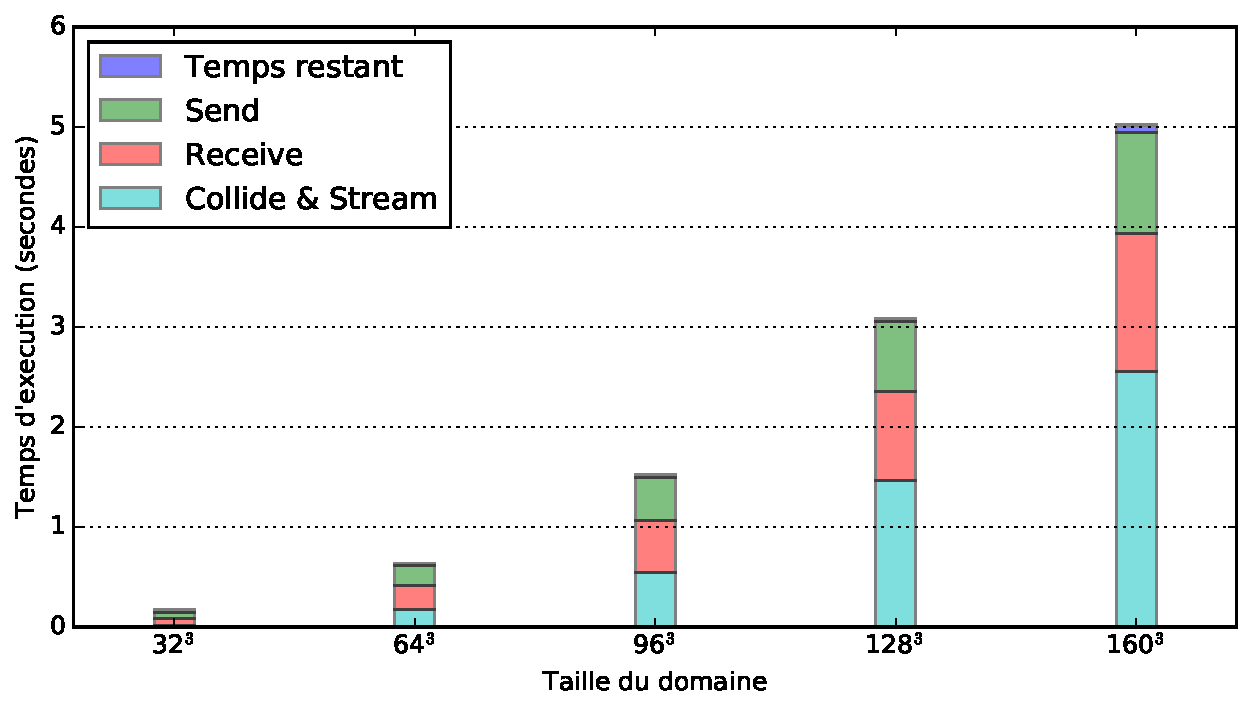
\includegraphics[fbox, scale=0.57]{images/perfs/lbm_simple_lbmcuda/time/repartition/tesla-opt-64.pdf}
		\label{fig:gpu_rep_times_tesla}
	}
	\caption{Profil des temps d'exécution sur un \acs{GPU}}
	\label{fig:gpu_rep_times}
\end{figure}

\begin{figure}[h]
	\centering
	\subfigure[\acs{GPU} Pascal]{%
		\centering
		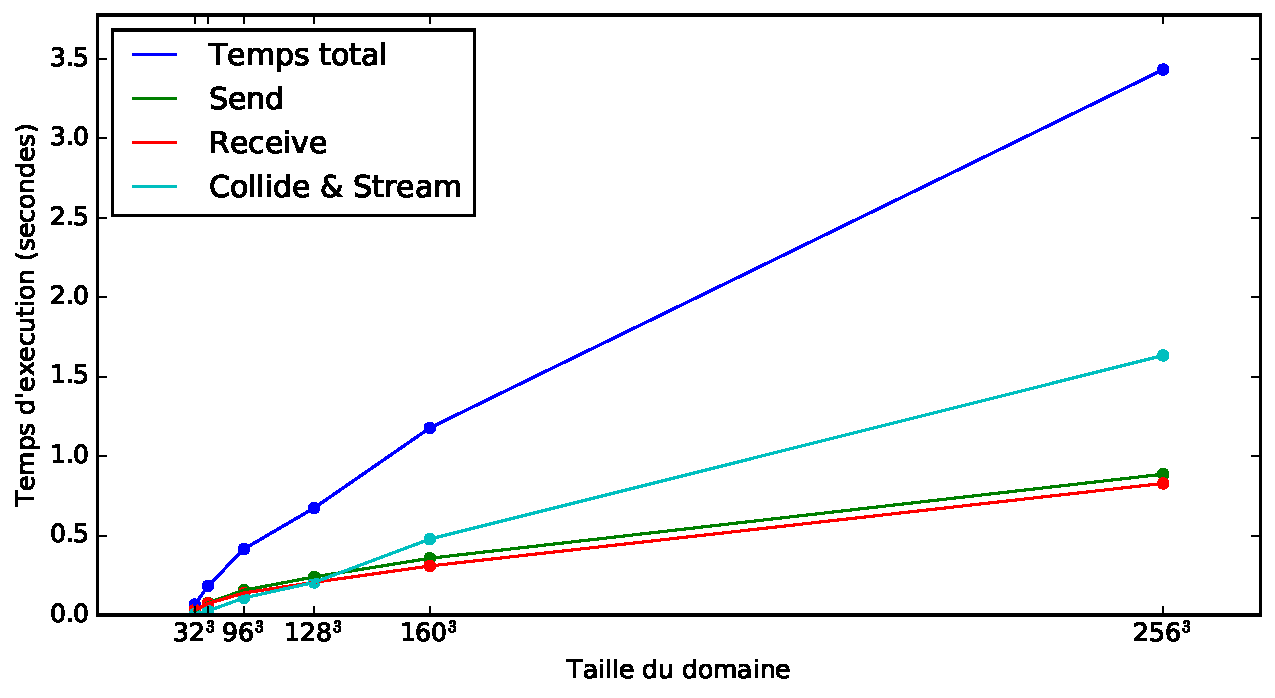
\includegraphics[fbox, scale=0.57]{images/perfs/lbm_simple_lbmcuda/time/curve/pascal-opt-64.pdf}
		\label{fig:gpu_curve_times_pascal}
	}
	\subfigure[\acs{GPU} Titan]{%
		\centering
		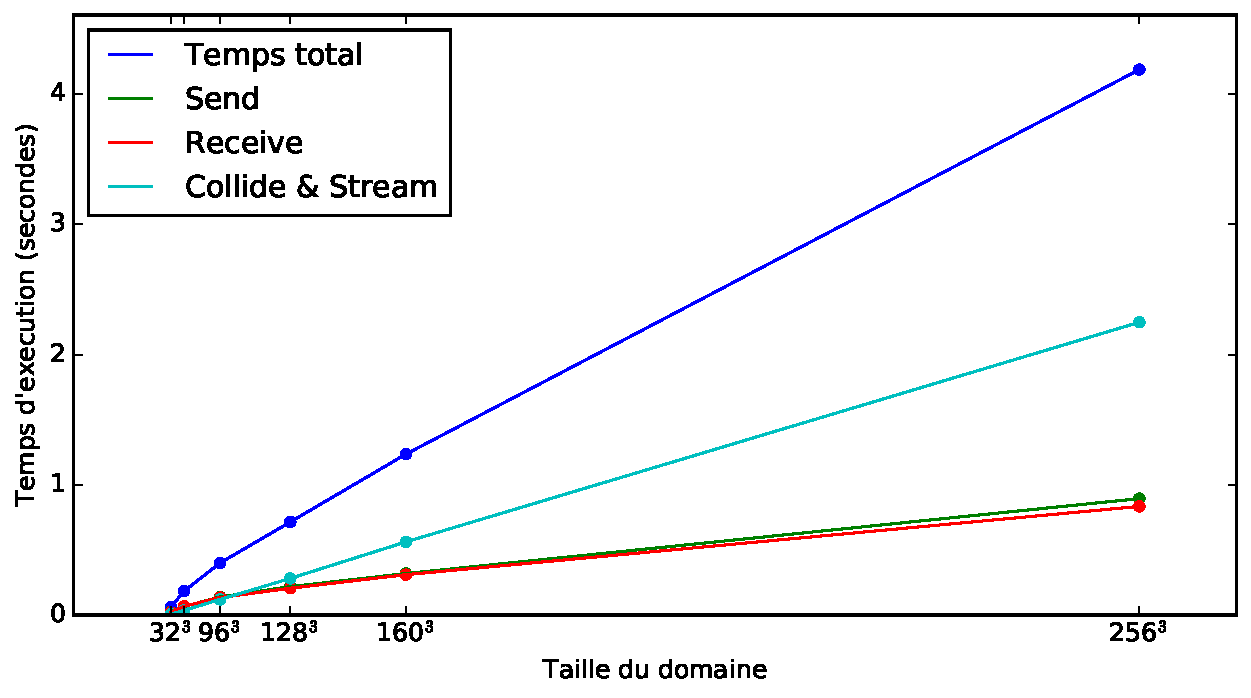
\includegraphics[fbox, scale=0.57]{images/perfs/lbm_simple_lbmcuda/time/curve/titan-opt-64.pdf}
		\label{fig:gpu_curve_times_titan}
	}
	\subfigure[\acs{GPU} Tesla]{%
		\centering
		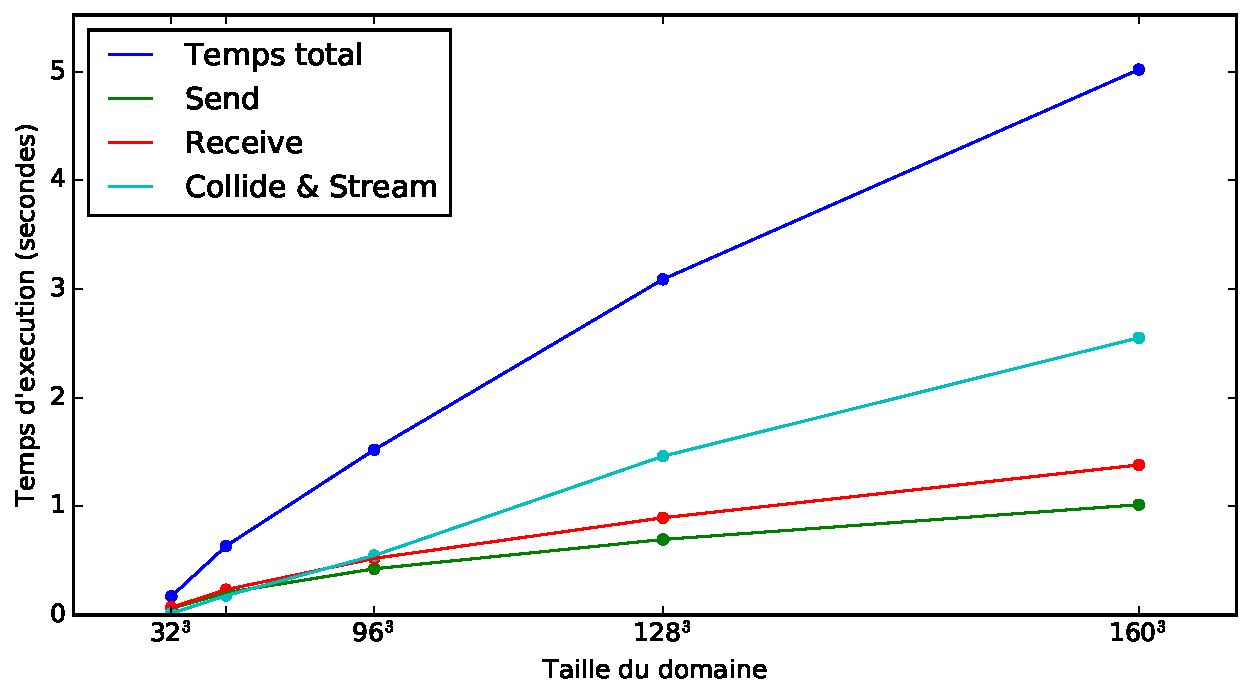
\includegraphics[fbox, scale=0.57]{images/perfs/lbm_simple_lbmcuda/time/curve/tesla-opt-64.pdf}
		\label{fig:gpu_curve_times_tiesla}
	}
	\caption{Courbe des temps d'exécution sur un \acs{GPU}}
	\label{fig:gpu_curve_times}
\end{figure}

\section{\textit{Benchmarks} de l'implémentation hybride}

\subsection{Profilage d'exécutions séquentielles}
Maintenant que le profil des temps d'exécution est connu sur \acs{GPU}, cette section s'intéresse à celui d'une exécution hybride à l'aide de \texttt{cavity\_benchmark}. Les temps d'exécution sont calculés sur le même principe que ceux de la section \ref{title-profilage_gpu} mais considèrent en plus les \textit{Collide \& Stream} effectués par les sous-domaines de Palabos ainsi que la duplication des chevauchements (détaillé en section \ref{title-transfert_palabos_cp}). Les mesures sont effectuées sur le \acs{GPU} Pascal, qui montrent jusqu'ici les meilleures performances. 

Le domaine de $132^3$ \textit{lattices} est découpé en 27 sous-domaines (voir section \ref{title-cavity_benchmark}). Le sous-domaine central est calculé par le co-processeur et les autres par le \acs{CPU}. Deux séries de mesures, où sont comparé l'impact sur les performances des transferts complets ou partiels (détaillé en section \ref{title-transfert_palabos_cp}),  sont effectuées ; La première série utilise un co-processeur \acs{CPU} (figures \ref{fig:hybrid_rep_times_cpu}) à des fins de référence et la seconde un co-processeur \acs{GPU} (figures \ref{fig:hybrid_rep_times_gpu}).

\subsubsection{Méthode de transfert (complet/partiel)}
Cet  aspect a l'effet le plus flagrant sur les performances. Avec un co-processeur \acs{CPU}, le temps d'exécution général augmente avec la taille du domaine lors de transfert complet tandis qu'il reste stable avec des transferts partiels. Non seulement les temps de transfert complets sont nettement supérieurs, mais on observe aussi qu'une part inconnue du temps d'exécution de Palabos augmente; probablement pour gérer ce flux de données nettement supérieur. On retrouve ce comportement avec un co-processeur \acs{GPU}. Toutefois, on observe qu’avec la méthode de transfert partiel le temps de calcul diminue avec l’augmentation de la taille du sous-domaine central. La méthode de transfert complet est par conséquent à bannir, exception faite pour les très petits sous-domaines comme l'illustre la figure~\ref{fig:trsf_methods}. Mais comme l’explique la sous-section suivante, ces sous-domaines de petite taille sont à éviter de toute manière.

\subsubsection{Dimension des sous-domaines} \label{title-mesure_hybride_dim_sous_dom}
Comme l'illustre la figure \ref{fig:plb_full_vs_partial_transfert}, la taille de l'enveloppe d'un transfert partiel n'augmente que très peu, proportionnellement à la taille du sous-domaine. Le temps gagné par le \acs{GPU} à calculer une large partie du domaine n'est ainsi plus gâché par le temps nécessaire à son transfert. Pour se convaincre du gain, il suffit de comparer le temps que met le co-processeur \acs{CPU} (figure \ref{fig:hybrid_rep_times_cpu_partial}) et le co-processeur \acs{GPU} (figure \ref{fig:hybrid_rep_times_gpu_partial}) pour calculer le plus grand sous-domaine: la moitié du temps total contre une fraction du temps à peine visible respectivement.

Pourtant, si le temps de calcul est proportionnel à la taille des sous-domaines confiés aux \acs{CPU} de Palabos, celui-ci devrait être inférieur au temps observé par les mesures. En effet, si l’on calcule les proportions du domaine $p_{pa,}$ et $p_{gpu}$ attribuées au \acs{CPU} et \acs{GPU}, avec $D$ la taille du  domaine, $d_{gpu}$ la taille du sous-domaine attribué au \acs{GPU} et $d_{pal}$ la taille cumulée des sous-domaines attribués à Palabos:

\begin{align}
D &= 132^3 = 2299968\\
d_{gpu} &=128^3 = 2097152\\
d_{pal} &= D - d_{gpu} = 202816\\
p_{gpu} &= \frac{d_{gpu}}{D} \approx 0.912 \approx 91\% \\
p_{pal} &= \frac{d_{pal}}{D} \approx 0.088  \approx 9 \%
\end{align}

on trouve que seul $9\%$ du domaine est attribué au \acs{CPU}. Le temps de calcul devrait être près de $9\%$ de celui mesuré pour $d_{gpu}=8^3$. Or, il n'a diminué que d'un tiers environ. 

Ce comportement s'explique probablement par les dimensions des sous-domaines attribués à Palabos. En effet, les sous-domaines avec $d_{gpu}=128^3$ ressemblent à ceux illustrés sur la droite de la figure \ref{fig:decoupage_sous_domaine_cavity_benchmark}, mais nettement plus fins encore ! Dans cette configuration, l'accès mémoire à ces sous-domaines n'est probablement pas très optimal en raison de leurs dimensions. 

\subsubsection{Duplication des chevauchements}
Les mesures montrent la part non négligeable qu'occupe la duplication des chevauchements. Toutefois, elle reste stable, qu'importe la configuration des sous-domaines.

\subsubsection{Nombre d'itération}\label{title-iterations_palabos}
La section \ref{title-iterations} montre que les performances de l'implémentation sur \acs{GPU} ne sont pas influencées par le nombre d'itérations et celles de Palabos ne devraient pas l'être non plus. Toutefois, on ne peut pas écarter, a priori, la possibilité d'un mécanisme, caché dans l'architecture de Palabos, qui influencerait les performances au fil des générations.

Les mesures qu'illustre la figure \ref{fig:lups_by_iter_palabos} montrent cependant que les performances restent stables avec les itérations et écartent ainsi le doute sur la question.

\begin{figure}[H]
	\centering
	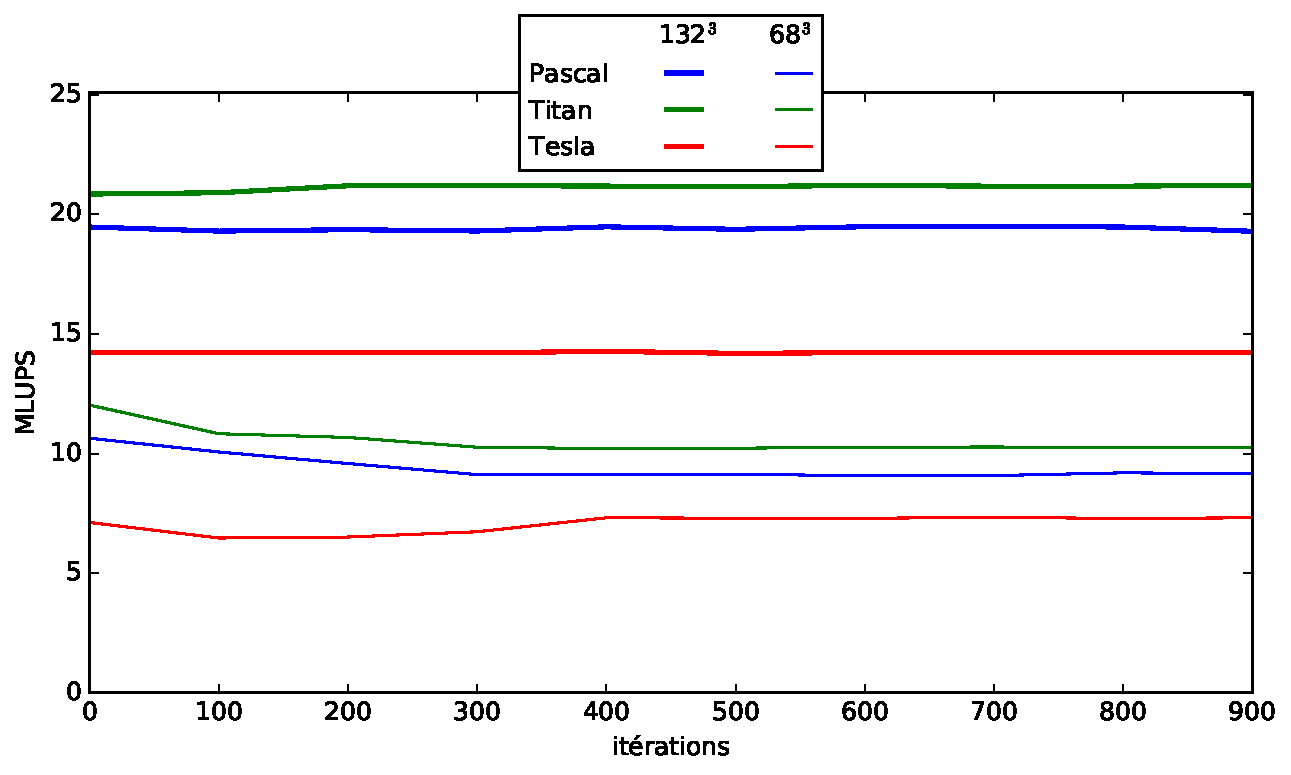
\includegraphics[fbox, scale=0.61]{images/perfs/cavity_benchmark/lups_by_iter.pdf}
	\caption{Performances en fonction du nombre d'itérations sur Palabos}
	\label{fig:lups_by_iter_palabos}
\end{figure}


\begin{figure}[h]
	\centering
	\subfigure[Tranfert complet]{%
		\centering
		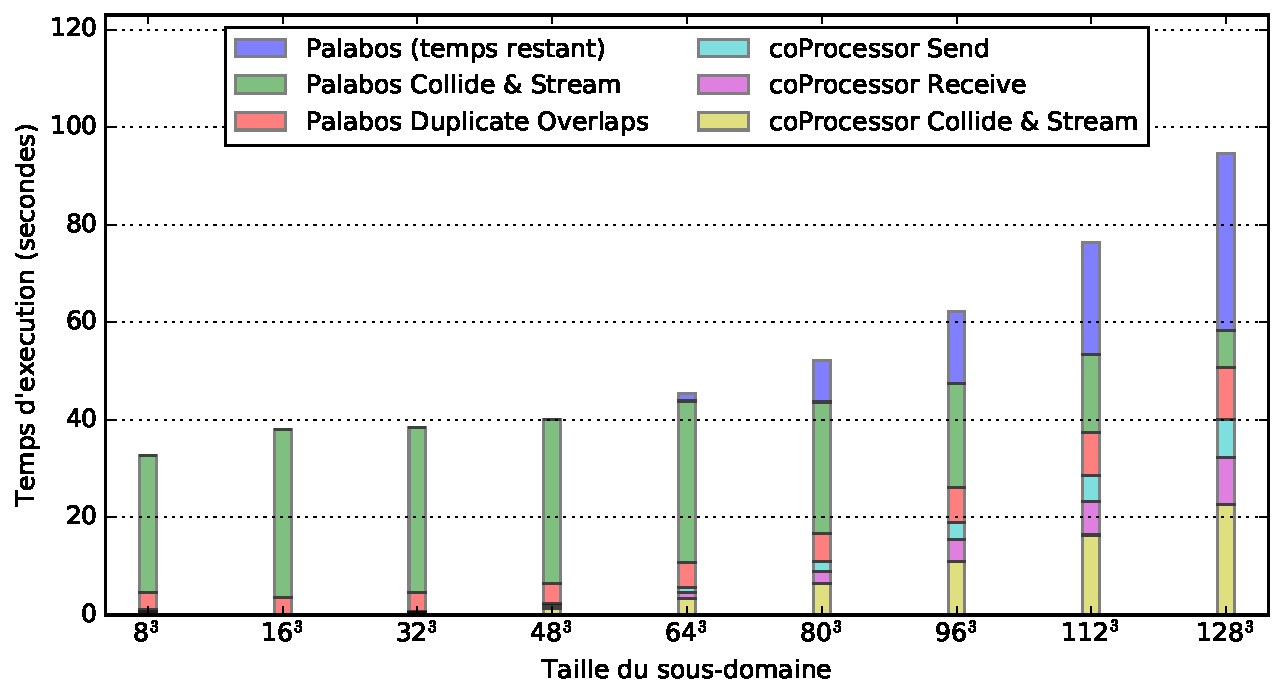
\includegraphics[fbox, scale=0.7]{images/perfs/cavity_benchmark/src_time_cpu_N132.pdf}
		\label{fig:hybrid_rep_times_cpu_full}
	}
	\subfigure[Transfert partiel]{%
		\centering
		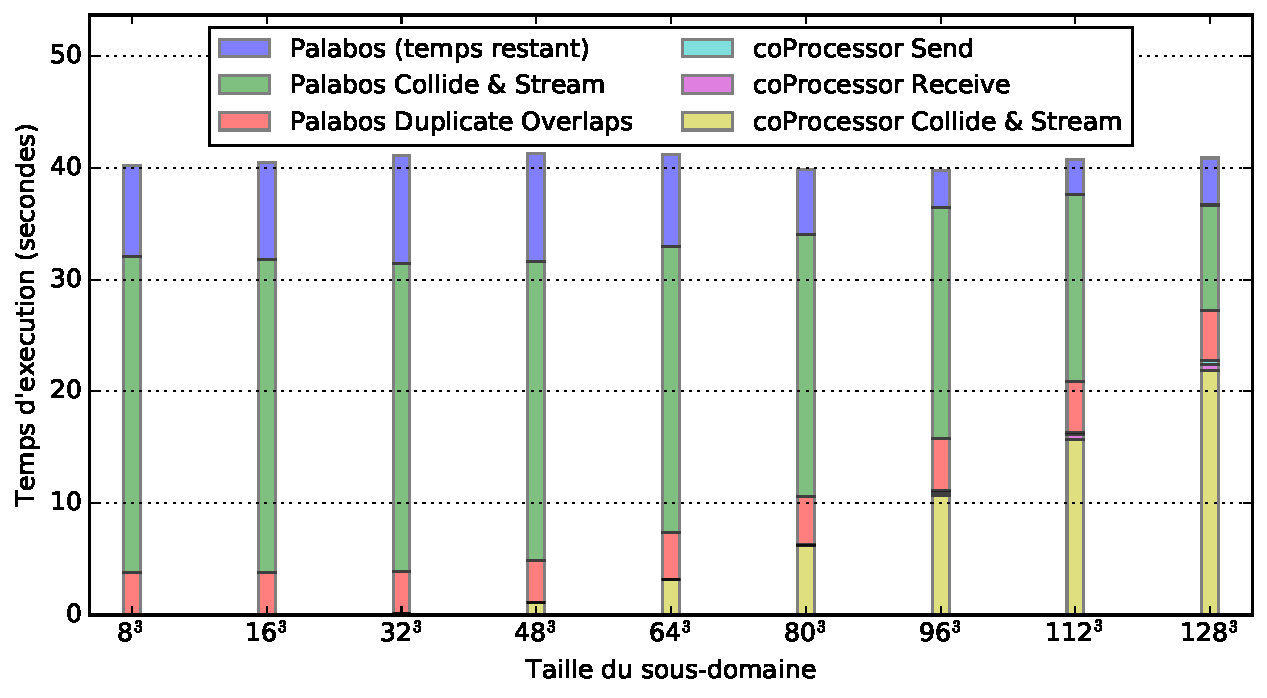
\includegraphics[fbox, scale=0.7]{images/perfs/cavity_benchmark/src_time_cpu_boundary_N132.pdf}
		\label{fig:hybrid_rep_times_cpu_partial}
	}
	\caption{Profil des temps d'exécution sur un co-processeur \acs{CPU}}
	\label{fig:hybrid_rep_times_cpu}
\end{figure}

\begin{figure}[h]
	\centering
	\subfigure[Tranfert complet]{%
		\centering
		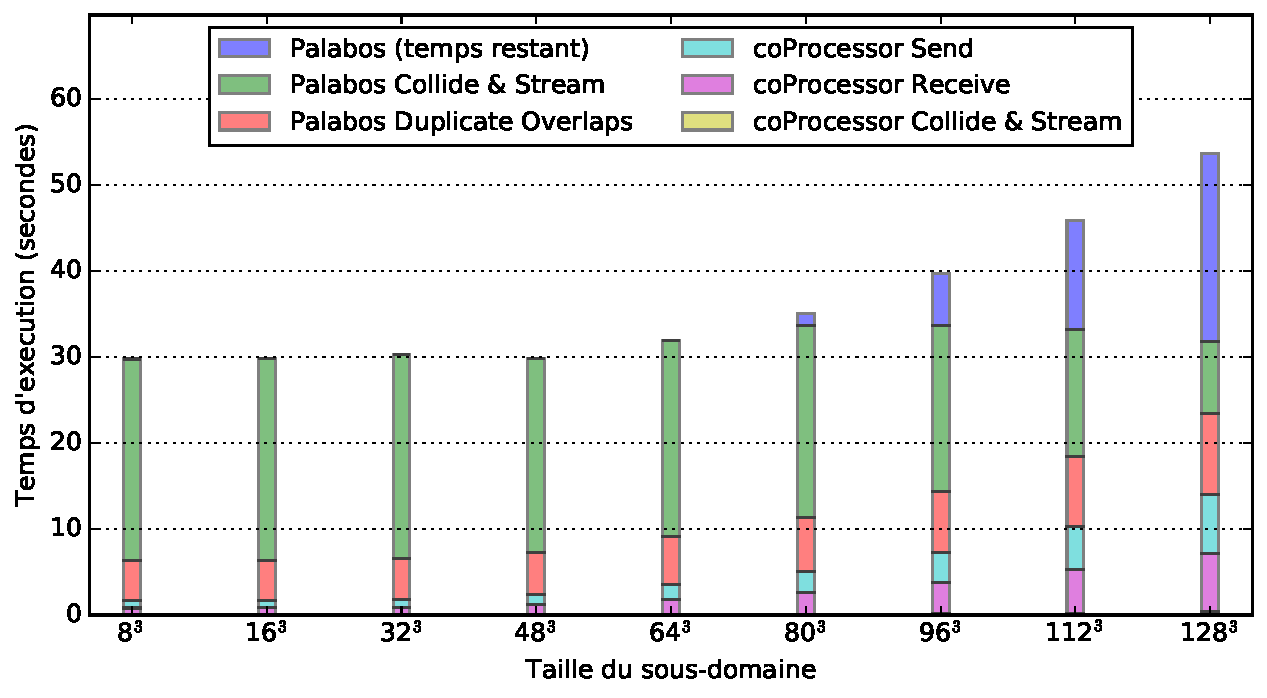
\includegraphics[fbox, scale=0.7]{images/perfs/cavity_benchmark/src_time_gpu_N132.pdf}
		\label{fig:hybrid_rep_times_gpu_full}
	}
	\subfigure[Transfert partiel]{%
		\centering
		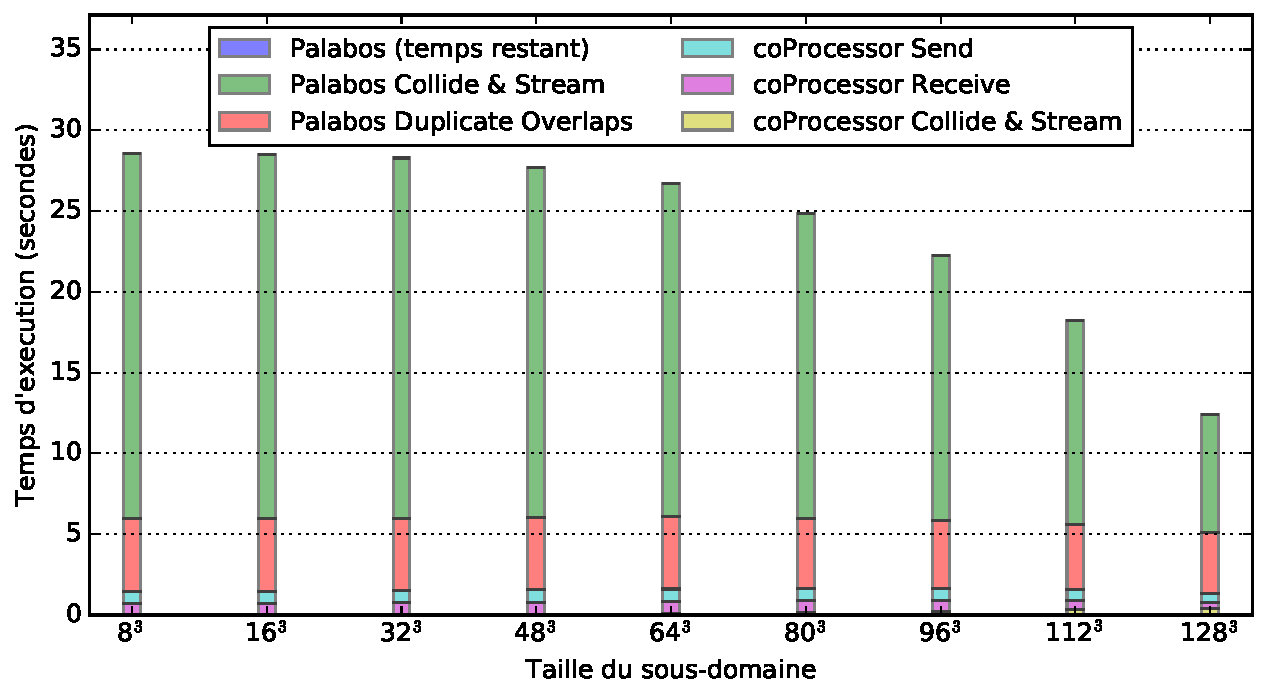
\includegraphics[fbox, scale=0.7]{images/perfs/cavity_benchmark/src_time_gpu_boundary_N132.pdf}
		\label{fig:hybrid_rep_times_gpu_partial}
	}
	\caption{Profil des temps d'exécution sur un co-processeur \acs{GPU}}
	\label{fig:hybrid_rep_times_gpu}
\end{figure}


\begin{figure}[h]
	\centering
	\subfigure[Co-processeur \acs{CPU}]{%
		\centering
		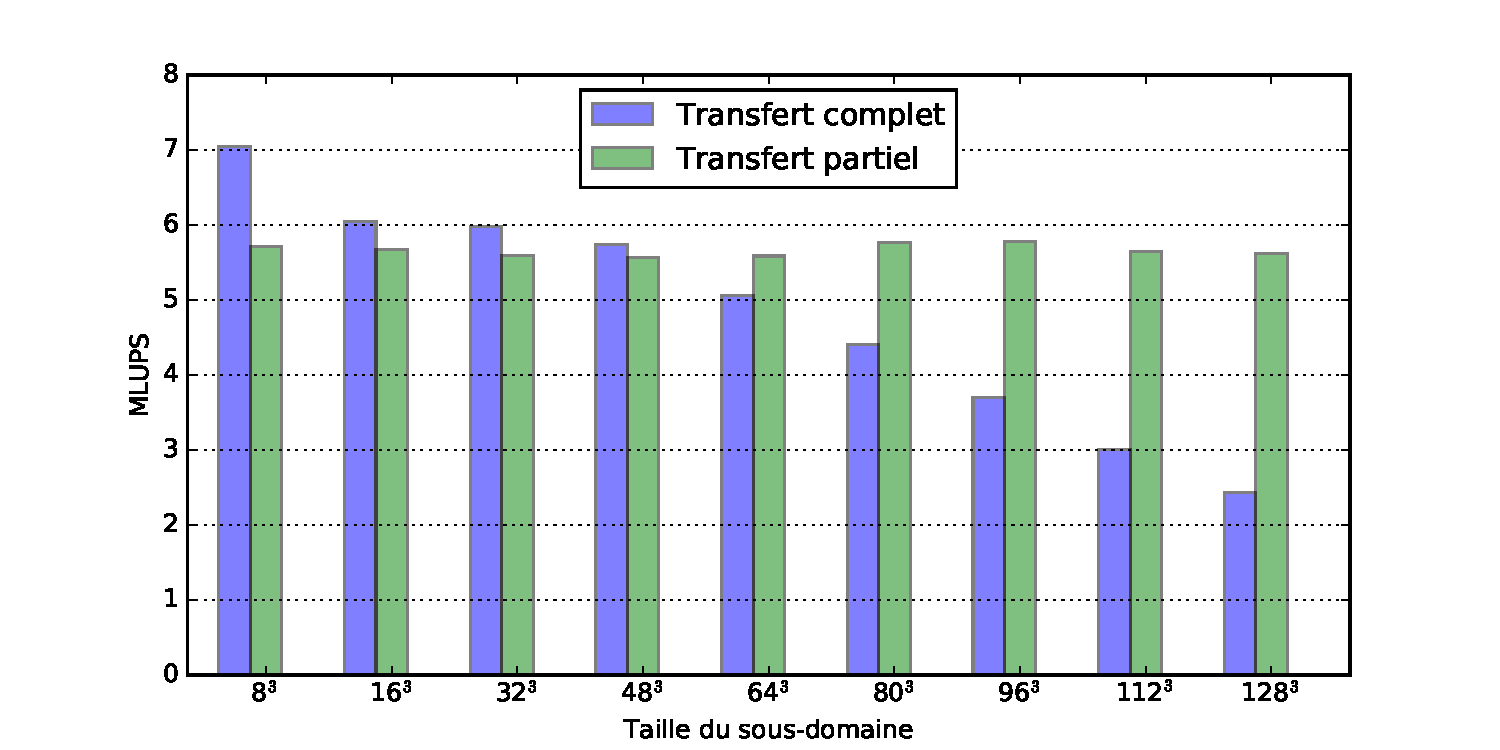
\includegraphics[fbox, scale=0.57]{images/perfs/cavity_benchmark/lbm_N132_full-vs-part_cpu.pdf}
		\label{fig:trsf_methods_cpu}
	}
	\subfigure[Co-processeur \acs{GPU}]{%
		\centering
		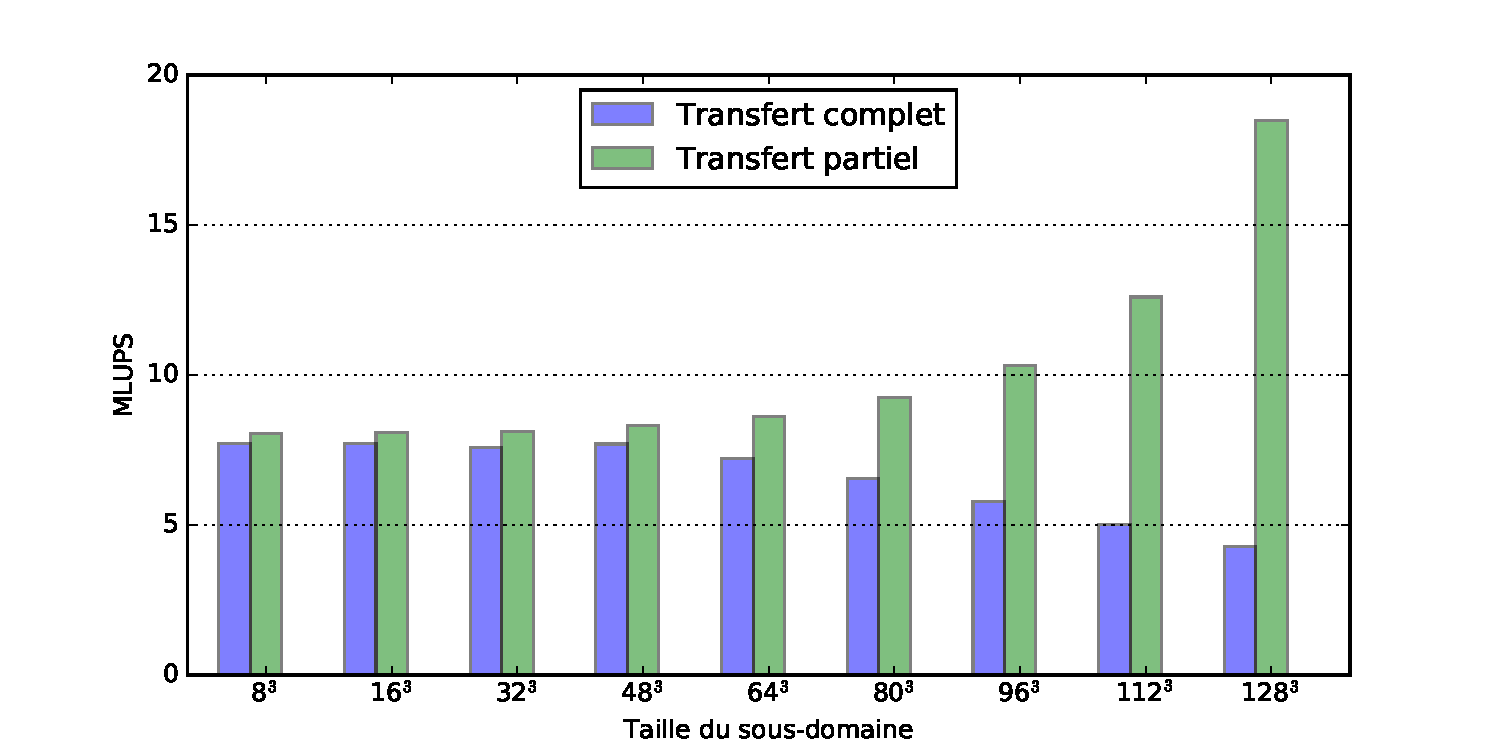
\includegraphics[fbox, scale=0.57]{images/perfs/cavity_benchmark/lbm_N132_full-vs-part_gpu.pdf}
		\label{fig:trsf_methods_gpu}
	}
	\caption{Performance des méthodes de transfert entre Palabos et le co-processeur}
	\label{fig:trsf_methods}
\end{figure}

\subsection{Exécutions parallèles}
Pour obtenir des performances intéressantes, Palabos permet de paralléliser les calculs des différents sous-domaines. Cette section analyse les performances d'exécutions parallélisées sur 9 \textit{threads}. Bien que l'idéale aurait été 27 \textit{threads} (soit un par sous-domaine), le \textit{cluster} de calcul ne permet pas d'en attribuer autant. Par conséquent, chaque \textit{thread} calcul trois sous-domaine séquentiellement sur le \acs{CPU}, à l'exception de l'un d'entre eux qui utilise le co-processeur sur le sous-domaine central. La figure~\ref{fig:perf_mpi} illustre les performances mesurées pour les exécutions hybrides avec les trois types de \acs{GPU} disponibles.

Bien que le \acs{GPU} le plus puissant soit Pascal, les meilleures performances parallèles sont obtenues sur Titan qui est doté de \acs{CPU} plus rapides (voir la table \ref{table:gpu_specs}).

On observe sinon que les trois simulations suivent la même tendance. Les performances augmentent pour atteindre leur pic entre les dimensions $32^3$ et $48^3$ du sous-domaine du co-processeur puis diminue ensuite avec une très légère augmentation à $128^3$.

Le pic de performance semble coïncider avec la dimension à laquelle tous les sous-domaines ont la même taille, soit $\big(\nicefrac{132}{3}\big)^3 = 44^3$. Cette dimension assure une distribution équitable du travail entre tous les \textit{threads} (à l'exception de celui du \acs{GPU} qui serait plus rapide) et évite le problème évoqué en section \ref{title-mesure_hybride_dim_sous_dom} sur  les dimensions non optimales pour les \acs{CPU}. Cette tendance apparaît tant avec un co-processeur \acs{CPU} que \acs{GPU}, ce qui indique qu'elle est principalement due aux \acs{CPU}. La seule différence (discrète) avec le \acs{GPU} est la légère augmentation de performance que l'on devine sur $128^3$, qui parviendrait probablement à tirer les performances vers le haut à partir de ce point, s'il pouvait s'occuper d'un sous-domaine plus grand.
  
\begin{figure}[h]
	\centering
	\subfigure[\acs{GPU} Pascal]{%
		\centering
		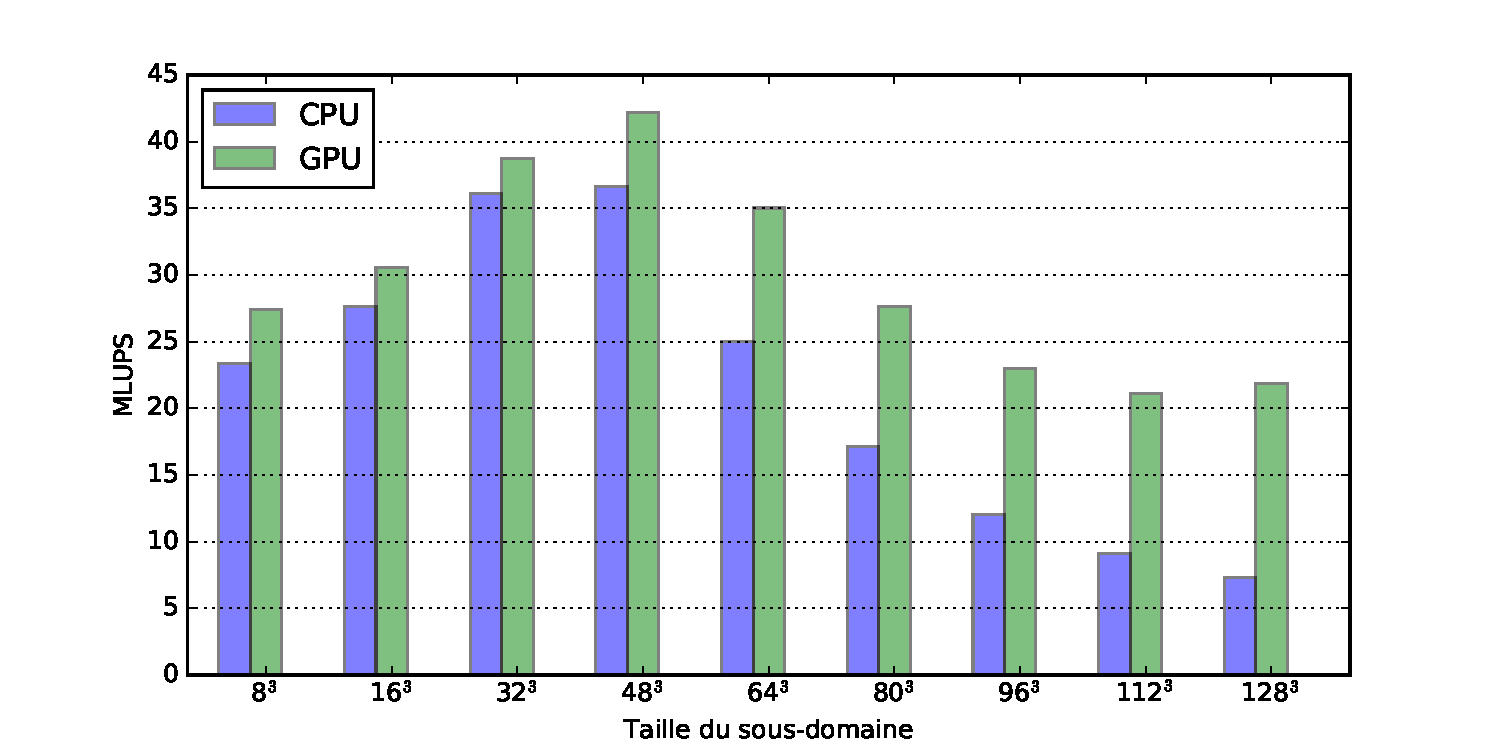
\includegraphics[fbox, scale=0.54]{images/perfs/cavity_benchmark/lbm_N132_pascal_mpi_9_cpu-vs-gpu.pdf}
		\label{fig:perf_mpi_pascal}
	}
	\subfigure[\acs{GPU} Titan]{%
		\centering
		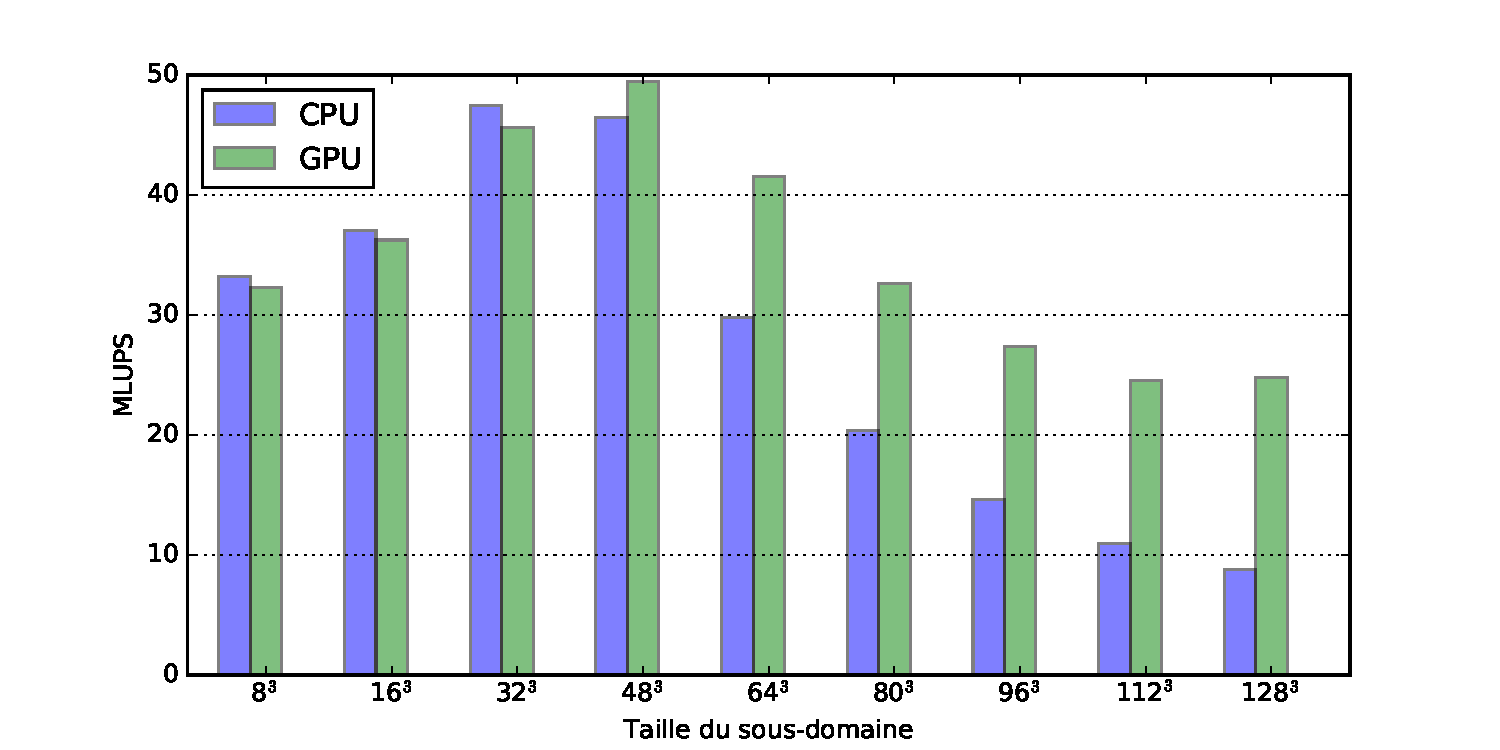
\includegraphics[fbox, scale=0.54]{images/perfs/cavity_benchmark/lbm_N132_titan_mpi_9_cpu-vs-gpu.pdf}
		\label{fig:perf_mpi_titan}
	}
	\subfigure[\acs{GPU} Tesla]{%
		\centering
		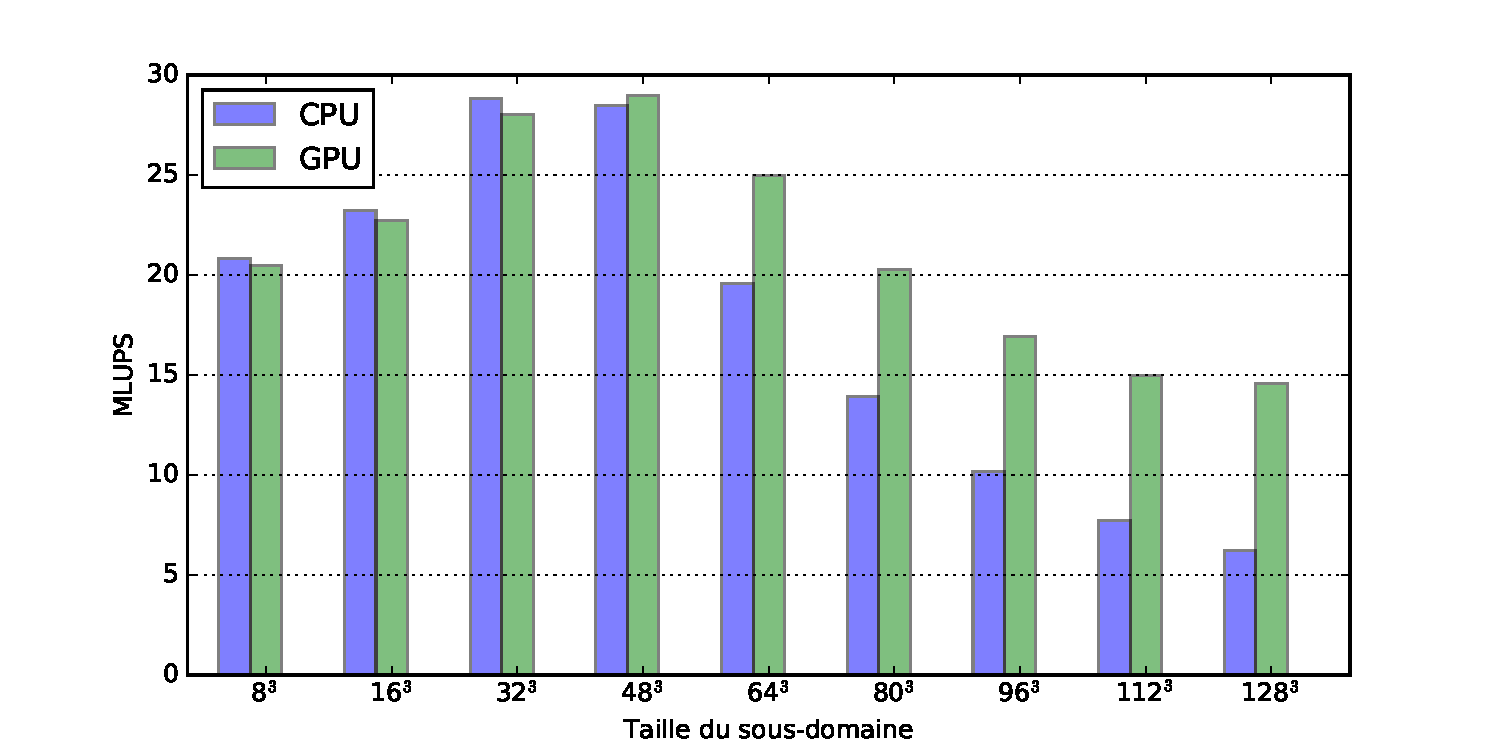
\includegraphics[fbox, scale=0.54]{images/perfs/cavity_benchmark/lbm_N132_tesla_mpi_9_cpu-vs-gpu.pdf}
		\label{fig:perf_mpi_tesla}
	}
	\caption{Performance d'exécutions parallèles sur 9 \textit{threads}}
	\label{fig:perf_mpi}
\end{figure}

